%\documentclass[12pt,letter]{report}
\documentclass[12pt,oneside,openany,letter]{book}
\usepackage[colorlinks=true,bookmarksnumbered,linktocpage,pdftex]{hyperref}
\usepackage{hyperref}
\usepackage[activeacute,spanish]{babel}
\usepackage[utf8]{inputenc}
\usepackage{amsmath}
\usepackage{float}
\usepackage{epsfig}
\usepackage{siunitx}
\usepackage{graphicx}
\usepackage{titlesec}
\usepackage{multirow}
\usepackage{graphicx}
\usepackage{caption}
\usepackage{subcaption}
\usepackage{color}
\usepackage{calc}
\usepackage[nottoc]{tocbibind}
\usepackage{titletoc}
\usepackage{capt-of}
\usepackage{verbatim}
\usepackage[natbibapa]{apacite}
\usepackage[titletoc,title]{appendix}
\usepackage[left=3cm, right=3cm,top=3cm, bottom=2.5cm]{geometry}

\newcommand{\bigrule}{\titlerule[1mm]}
\definecolor{c1}{rgb}{0,0.5,0}
\definecolor{c2}{rgb}{0.9,.0,0}
\definecolor{c3}{rgb}{.465,.535,.605}%color del panel
\definecolor{c4}{rgb}{.6,.6,.6}%color de los botones del panel

\hypersetup{linkcolor=blue}                         
\hypersetup{citecolor=red}

%%%%FORMA DE LOS CAPITULOS SECCIONES...ETC%%%%%%

%========================================
% Formato de capítulos y secciones
%\newcommand{\esp}{\rule{0in}{3ex}} %para crear espacios en las tablas
\usepackage{titlesec}
\titleformat{\section}[hang]{\bfseries} {\Large\thesection}{12pt}{\Large}[{\titlerule[0pt]}]
 % Para hacer una línea debajo de cada sección
\titleformat{\chapter}[display] % cambiamos el formato de los capítulos
{\bfseries\Huge} % por defecto se usarán caracteres de tamaño \Huge en negrita
{ \filleft % texto alineado a la derecha
 \Large\chaptertitlename\ % "Capítulo" o "Apéndice" en tamaño \Large en lugar de \Huge
 \Large\thechapter} % número de capítulo en tamaño \Large
{0mm} % espacio mínimo entre etiqueta y cuerpo
{\filleft} % texto del cuerpo alineado a la derecha
[\vspace{0.5mm} \bigrule] % después del cuerpo, dejar espacio vertical y trazar línea horizontal gruesa



\setlength{\parskip}{10pt} %espacio entre párrafos
\makeatletter
\newcommand\figcaption{\def\@captype{figure}\caption}
\makeatother


%%%%%%%%%% NEW COMANDS %%%%%%%%%%%%%%%%%%%%%%%%%%%%%%%%%%%%%%%%%55

%%%%%%%%%%%%%%%%%%%%%%%%%%%%%%%%%%%%%%%%%%%%%%%%%%%%%%%%%%%%%%%%%%%%%%%%%%%%%%
\parindent0cm %Sangria
\parskip0.5cm %Espacio entre prrafos.
\baselineskip0.5cm
\begin{document}

\begin{titlepage}
%\bce
\centering {\Large {\sc  Estudio del último eclipse cromosférico de $\zeta$  Aurigae, otoño 2019}}

\vfill

\centering {\Large \sc Natalia Lucía Oliveros Gómez$^{1,2}$}

\vfill

\centering {\Large \textbf{Director:} Ph.D Klaus-Peter Schröder $^{3}$}

\centering {\Large \textbf{Codirector:} Ph.D Luis Alberto Núñez$^{1,2}$}

\centering {\Large \textbf{Codirector:} M.Sc Faiber Danilo Rosas$^{3}$}

\vfill

\centering {\Large {Trabajo de grado para optar al t\'itulo de Física}}


\vfill
{\Large $^1$ Grupo de Investigaci\'on en Relatividad y Gravitaci\'on - UIS} \\
{\Large $^2$ Grupo Halley de Astronom\'ia y Ciencias Aeroespaciales} \\
{\Large $^3$ Grupo de Investigación en Física Estelar, Universidad de Guanajuato}

\vfill

\centering {\Large Universidad Industrial de Santander\\Facultad de
Ciencias\\Escuela de F\'{i}sica\\2021}
\end{titlepage}
\newpage

%%%%%%%%%%%%%%%%%%%%%%%%%%%%%%%%%%%%%
%%%%%%%%% dedicado a %%%%%%%%%%%%%%%%
%%%%%%%%%%%%%%%%%%%%%%%%%%%%%%%%%%%%%
\newpage
%\pagenumbering{Roman}
%\pagestyle{empty}
\begin{flushright}
\vspace{5 cm}
\textit{A Roger, Olga, \\
mi hermana y mi bella sobrina.\\
%Dedicado a todos los aspies\\ 
Para que nunca se rindan \\
y encuentren su lugar en este mundo.\\
En memoria de mi abuela,\\
Alicia Chacón.\\}

\begin{comment}
Dedicado a mi abuelita que me inspiró a soñar y aunque hoy no me verá graduada, estaría muy orgullosa de mí. También a mi familia que me apoyó aunque inicialmente consideraron las ciencias como una carrera absurda, pero hoy lo aprecian con ojos de asombro e inspiración para aprender cada día un poco más.
\end{comment}

\vspace{0.5cm}

\end{flushright}

\chapter*{Agradecimientos}

\begin{comment}
\noindent Gracias a mi familia\footnote{Roger Oliveros, Olga Gómez, Catherine Oliveros} porque a pesar de quererme cerca a ellos, me comprenden y me extrañan con felicidad de que haga lo que me gusta, aprender del mundo y mucho más allá de lo que no podemos ver con nuestros ojos. A Dios y/o al universo  por permitirme la vida y coincidir en espacio y tiempo con personas maravillosas que han hecho de mi vida momentos más agradables. Como mis compañeros y amigos de carrera\footnote{Steven Rico, Rolando Carvajal, Juan Manuel Pacheco y Laura Mártinez}, a aquellos se convirtieron en mi otra familia\footnote{Grupo Halley UIS}  con el transcurso de los años. 

\noindent A los profesionales que me formaron como una persona integra, no solo académicamente sino para ser mejor persona. A mi codirector\footnote{Luis Núñez}, quien ha sido mi padre académico y quien desde que estaba en mi primer año de carrera me permitió el acercamiento a la astronomía. A quienes me acompañaron\footnote{Jose Luis Salamanca} a plantear formas óptimas de resolver problemas. 


\noindent También a que el mundo es tan pequeño que de una forma u otra\footnote{Lauren Flor} terminaría conociendo a mi director \footnote{Klaus-Peter Schröder} y codirector \footnote{Faiber Danilo Rosas} que me permitieron hacer parte de su universidad, por su guía excepcional en este trabajo, aumentando mi pasión por la astronomía y alimentar mi curiosidad de conocer las estrellas. Gracias a todo el grupo de investigadores del TIGRE, por permitirme ser parte de su excelente grupo de investigación internacional.
\end{comment}




\tableofcontents
\listoffigures
%\listoftables
%\newpage
\chapter*{Resumen}
{\footnotesize \textbf{T\'ITULO:} ESTUDIO DEL ÚLTIMO ECLIPSE CROMOSFÉRICO DE $\zeta$ AURIGAE, OTOÑO 2019.\\
\textbf{AUTORA:} NATALIA LUCÍA OLIVEROS GÓMEZ\\
\textbf{PALABRAS CLAVE:} Sistemas binarios, cromosfera, espectroscopía, densidad de masa columnar, curvas de crecimiento.
\vspace{2mm}

Debido a la importancia de los sistemas binarios en la astrofísica, los cuales proveen con precisión cantidades físicas que permiten un conocimiento amplio de la dinámica estelar y la evolución de las estrellas. En el presente proyecto se realiza un análisis de la variación de la densidad de masa columnar con la altura en la cromosfera de la estrella principal del sistema binario $\zeta$ Aurigae durante el eclipse observado en otoño de 2019. Se hace un estudio de la variabilidad temporal de la línea de calcio ionizado K de CaII (3934 \r{A}), usando espectros con relación S/N de 200-300 y resolución de $\sim$ 20000 obtenidos por TIGRE-HEROS; con lo cual se generan curvas de crecimiento para hacer un análisis de la cromosfera que al ser comparado con eclipses anteriores del mismo sistema, durante la estancia se busca proponer un modelo que explique el cambio de densidad de masa columnar con la altura en la cromosfera de la estrella gigante y la dinámica del sistema.}

\chapter*{Abstract}

{\footnotesize \textbf{TITLE:} STUDY OF THE LAST CHROMOSPHERIC ECLIPSE OF $\zeta$ AURIGAE, AUTUMN 2019

\textbf{AUTHOR:} NATALIA LUCÍA OLIVEROS GÓMEZ.

\textbf{KEY WORDS:} Binary systems, chromosphere, spectroscopy, columnar mass density, growth curves.
}



%%%%%%%%%%%%%%%%%%%%%%
%%%%% CHAPTER 1  %%%%%
%%%%%%%%%%%%%%%%%%%%%%
\chapter{Introducción}\label{cap1}
La fotometría y espectroscopia son herramientas que permiten conocer información astrofísica, como propiedades estelares fundamentales, que para el caso de estrellas binarias, específicamente las eclipsantes, se pueden tener con mayor precisión que en estrellas individuales. Esto, debido a los fenómenos que pueden ser observados durante los eclipses, como es el caso de las cromósferas estelares. Así que sistemas como $\zeta$ Aurigae \citep{shenavrin2011vizier}, que hace parte de un grupo selectivo de sistemas binarios compuestos por una estrella gigante fría y una en secuencia principal caliente permiten el estudio de cromósferas. 
\vspace{2mm}

\noindent En trabajos anteriores ya se han hecho análisis tanto en fotometría como espectroscopia de Zeta Aurigae, con datos observacionales desde tierra y también con datos del IUE (International Ultraviolet Explorer) y HTS (Hubble Telescope Space) para conocer la geometría del sistema \citep{kps9} y algunas características de la variación de la densidad de masa \citep{kps1O} a partir de curvas de crecimiento \citep{complete}. Sin embargo, no todas las conclusiones de este sistema han sido satisfactorias, aún hay preguntas sin responder como si es posible relacionar los hallazgos de estrellas gigantes en un sistema binario con estrellas individuales, teniendo en cuenta las huellas evolutivas \citep{schroder1997critical}. Por lo que sigue siendo relevante el estudio de estos sistemas binarios.

\noindent Otra de las conclusiones relevantes y que se tendrán en cuenta en este proyecto es el análisis de la densidad de masa columnar con relación a algunos metales presentes en la atmósfera de estrellas gigantes. Por lo que surge la pregunta de ¿Cómo varía la densidad de masa columnar con la altura a medida que transcurre el eclipse de un sistema binario y si es posible con esto conocer la dinámica estelar? 


\noindent Al responder esta pregunta, se podría confirmar la veracidad de investigaciones anteriores que se han hecho a partir del análisis del sistema $\zeta$ Aurigae. Como conocer la altitud  y proyecciones geométricas de la posición de la estrella en secuencia principal según la fecha de ingreso y el valor obtenido de densidad de masa columnar.
\vspace{2mm}

\noindent A partir de conocer la densidad de masa columnar es posible relacionar los fenómenos físicos producidos en el interior de la atmósfera, para conocer la dinámica estelar; con la herramienta de espectroscopia se pueden conocer las interacciones fotón-átomo, átomo-átomo que incluye tipos de absorción, dispersión de resonancia, emisión (re-emisión). Donde cabe resaltar el papel de la teoría atómica al analizar los cambios en la atmósfera estelar (por procesos de ionización, resonancia, entre otros). Y además es bueno cuestionarse si posible relacionar estos procesos con la teoría electromagnética.

\begin{comment}
\noindent Al responder esta pregunta, inicialmente se podría confirmar la veracidad de investigaciones anteriores que se han hecho a partir del análisis del sistema $\zeta$ Aurigae. Actualmente se tiene la ecuación (\ref{perfil-densidad}) para los perfiles de densidad $n$, los cuales dependen de la altura $h$ de la atmósfera estelar, de acuerdo a las conclusiones de este trabajo se podrá confirmar o hacer aportes para mejorar las conclusiones actuales sobre este modelo. 

\begin{equation}
    n(h) = n_0 exp (-h/\alpha)
    \label{perfil-densidad}
\end{equation}
\vspace{2mm}

\noindent A partir de dicho modelo de densidad de masa columnar es posible relacionar los fenómenos físicos producidos en el interior de la atmósfera, para conocer la dinámica estelar; con la herramienta de espectroscopia se pueden conocer las interacciones fotón-átomo, átomo-átomo que incluye tipos de absorción, dispersión de resonancia, emisión (re-emisión), también la transferencia radiativa es indispensable al observar el proceso durante el paso de la radiación por la atmósfera de una estrella; adicionalmente cabe resaltar el papel de la teoría atómica al analizar los cambios en la atmósfera estelar (por procesos de ionización, resonancia, entre otros). Por otro lado, también es posible relacionar estos procesos con la teoría electromagnética.
\end{comment}
\vspace{2mm}

\noindent Una de las ventajas de este proyecto, para una mejor aplicación del método científico es que no solo se tienen en cuenta los conceptos físicos y de teoría estelar, sino que también se cuenta con datos observacionales, tomados del telescopio TIGRE \citep{schmitt2014tigre} con resolución espectral $\approx 21000$ y relación S/N $200-300$. Por lo tanto al relacionar la rama teórica y observacional se puede obtener un modelo que cumpla con ambas partes, haciendo esta investigación la más preciso posible.

\noindent Finalmente, además de implementar el método científico se está realizando la revisión de proyectos anteriores, logrando la caracterización del estado del arte en este tema, lo que permite un aprendizaje de conceptos fundamentales en física estelar, con un primer acercamiento a herramientas computacionales de la astronomía; permitiendo llegar a conclusiones relevantes en el área.

\section{Objetivos}

%%%%%%%%%%%%%%%%%%%%%%%%%%%%%%%%%%%%%%%%%%%%%%%%%%%%%%%%%%%%%%%%%%%%%%%%%%%%%%%%%%%%%%%%%%%%%
\subsection{Objetivo General}

Comparar la absorción cromosférica y el cambio de la densidad de columna N(h) del eclipse del sistema binario $\zeta$ Aurigae de otoño 2019 con un antiguo eclipse de 1987.


\subsection{Objetivos Espec\'ificos}
\begin{enumerate}
    \item Identificar líneas espectroscópicas presentes en la estrella gigante fría
    \item Obtener el espectro de las líneas de absorción cromosférica
    \item Cuantificar el valor del ancho equivalente ($W_{\lambda}$) de las líneas claves (Fe I, Ti II)  y encontrar las fuerzas del oscilador ($loggf$)

    \item Analizar las \textit{curvas de crecimiento} observacionales y teóricas

    \item Deducir la densidad de masa columnar
\end{enumerate}


%%%%%%%%%%%%%%%%%%%%%%
%%%%% CHAPTER 2  %%%%%
%%%%%%%%%%%%%%%%%%%%%%
\chapter{Estrellas}\label{cap2}
%%%%%%%%%%%%%%%%%%%%%%%%%%%%%%%
%%%%%%%%%   Section   %%%%%%%%%
%%%%%%%%%%%%%%%%%%%%%%%%%%%%%%%

\section{Sistemas binarios}

Los sistemas de estrellas binarios son  mucho más comunes en el Universo que las estrellas solitarias como nuestro sol, según \citep{fisher2005local}. Pero son muy interesantes y necesario porque nos permiten conocer información astrofísica, como la masa estelar y un radio de estado evolutivo con una precisión muy superior a la que es posible en el caso de las estrellas individuales, por lo que es relevante su investigación, además se pueden analizar sesiones de las estrellas como las cromósferas que solo se conoce para estos sistemas y existe la posibilidad de que estos resultados se puedan extrapolar a otras estrellas del mismo tipo, pero individuales; permitiendo avances en el conocimiento de atmósferas estelares y evolución estelar. Aún así, existen diferentes tipos de sistemas binarios, los cuales se clasifican de acuerdo a características observacionales, como la geometría, la relación de masas, la luminosidad, entre otras.

\noindent Algunos de los sistemas más representativos se nombran a continuación, sin embargo para este estudio solo en uno de estos. Los sistemas \textit{dobles ópticos} son estrellas que se encuentran en la misma línea de visión pero no están unidas gravitacionalmente.  Las \textit{binarias visuales} son aquellas que muestran parámetros comunes, pero se pueden resolver de manera independiente, estos sistemas proporcionan información relevante de la separación angular entre las componentes y el centro de masa; de estos también se desprenden las \textit{binarias astrométricas}, donde normalmente solo se ve una de las componentes estelares pero hay un movimiento aparente periódico en ella, permitiendo conocer la presencia de la otra. También están las \textit{binarias espectroscópicas}, las cuales se analizan a partir de espectros, donde hay desplazamientos periódicos en las líneas características y normalmente estan tan juntas como para observarse en una misma imagen.

\section{Sistemas binarios eclipsantes}
Las \textit{binarias eclipsantes}, son aquellas estrellas que se eclipsan mutua y periódicamente, que tienen planos orbitales orientado aproximadamente a lo largo de la línea de visión del observador. Se pueden observar a partir de fotometría con curvas de luz, donde cambia la magnitud aparente del sistema y con esto mismo obtener parámetros orbitales y propios de cada componente estelar, como temperaturas y radios relativos.

\noindent Con los eclipses se puede hacer una buena estimación de la inclinación $i$, cuando la distancia entre las estrellas es mayor a la suma de los radios de las estrellas involucradas. Esto se puede con ayuda de las curvas de luz, donde se aprecian las diferencias en luminosidad, las cuales se pueden relacionar con la inclinación y la  excentricidad orbital. Como se observa en la figura (\ref{fig:curva_luz}), al relacionarlo con la representación de los eclipses en la figura (\ref{representacion_eclipse}) se puede analizar la variación de las curvas de luz con respecto a la inclinación y las asimetrías en la curva se relacionan con la excentricidad.

\begin{figure}[h]
    \centering
    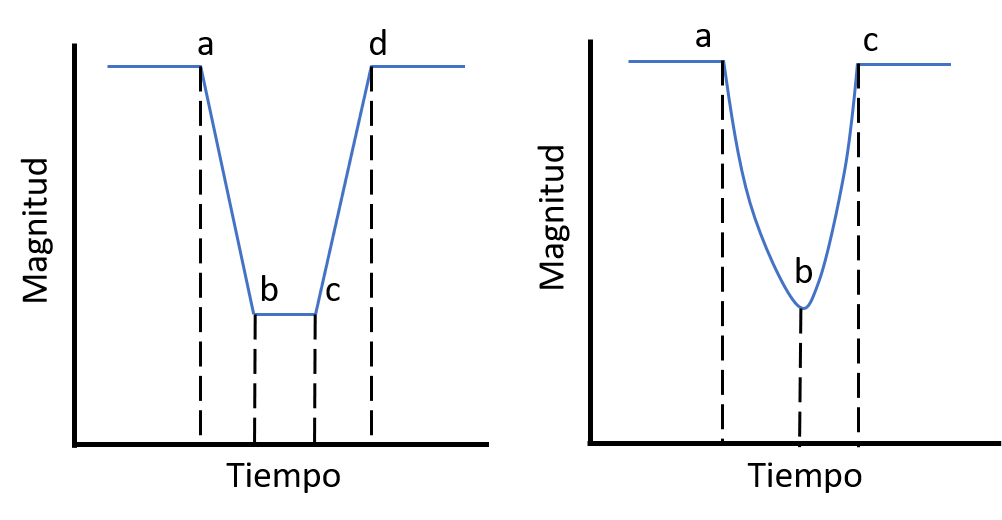
\includegraphics[width=0.65\linewidth]{Images/curvaluz.png}
    \caption{Representación de curvas de luz para dos casos con diferente inclinación del plano orbital respecto al observador}
    \label{fig:curva_luz}
\end{figure}


\begin{figure}[h]
    \centering
    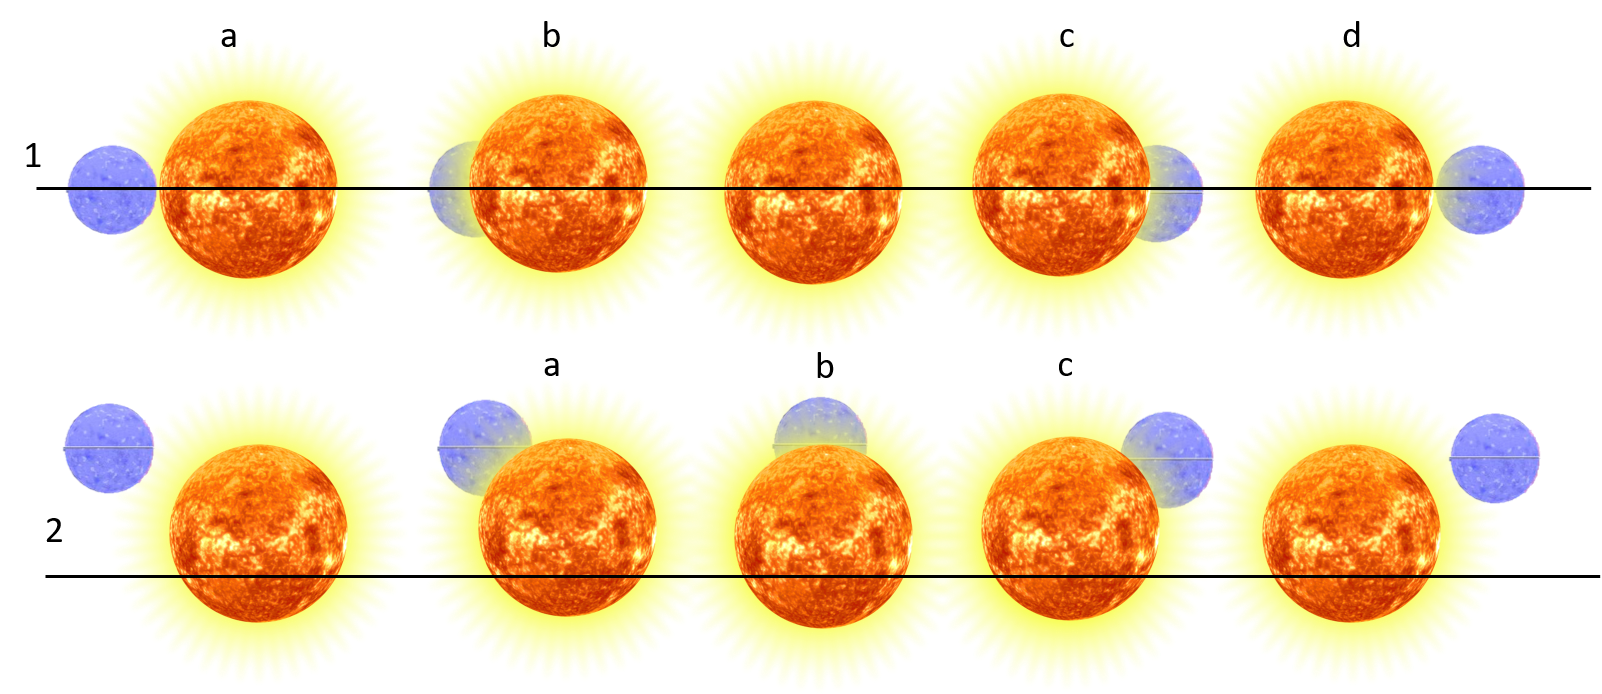
\includegraphics[width=1\linewidth]{Images/representacion_eclipse.png}
    \caption{Representación de un sistema binario eclipsante, sin tener en cuenta la geometría de algún sistema en específico, en el 1) se tiene una inclinación $i = 90^{o}$, 1a es el primer contacto, 1b es eclipse parcial entrante y 1c es el parcial saliente, entre 1b y 1c es el eclipse total y 1d es el cuarto contacto. 2) la inclinación es menor a $90^{o}$ }
    \label{representacion_eclipse}
\end{figure}

\noindent El énfasis de este proyecto es en un sistema binario eclipsante, compuesto por una estrella gigante y una caliente en secuencia principal, como este, hay sistemas muy característicos que se han usado para describir características físicas de estrellas, estos sistemas se conocen como \textit{Sistemas $\zeta$ Aur} \citep{ake2015giants} y desde la espectroscopia, siguiendo la figura (\ref{representacion_eclipse}), en primera instancia se tiene solo el espectro de la estrella gigante y a medida que se acerca la estrella compañera se obtiene un espectro compuesto por las dos estrellas (fig \ref{representacion_eclipse} 1a, 1b) debido a la superposición de cada componente estelar. El flujo de la gigante cada vez se hace más débil por la presencia de la compañera, sobre todo en la banda azul, donde hay absorción de la estrella compañera y se obtiene un aumento en la intensidad en su entrada. Es decir, \textit{la cromósfera absorbe selectivamente el calor} cuando la radiación de la estrella pasa por la línea de visión y a medida que pase por etapas cada vez más profundas, las líneas se van ensanchando obteniendo en el eclipse total solo el espectro de la estrella gigante. Y cuando va saliendo del eclipse total (fig \ref{representacion_eclipse} 1c, 1d) pasa esto mismo, pero en orden inverso. Por lo tanto si se tienen los espectros en orden temporal se observa la densidad de columna de la cromósfera a diferentes distancias de la extremidad de la estrella gigante y con esto se modelan gradientes de densidad y temperatura, obteniendo buenos modelos que se aproximen a lo que sucede en este proceso.

\subsection{Zeta ($\zeta$) Aurigae}

Este sistema binario fue descubierto en 1932 \citep{guthnick1934bevorstehende} y está compuesto por $\zeta$ Aur A, una gigante roja de tipo espectral K5II; y $\zeta$ Aur B una estrella de la secuencia principal de tipo espectral B7V \citep{shenavrin2011vizier}. Éste sistema se encuentra ubicado en la constelación de Auriga  y en él se presenta el fenómeno de eclipses atmosféricos, los cuales se pueden observar tanto de telescopios terrestres como en el espacio, ya que durante los eclipses la magnitud de $\zeta$ Aur A disminuye a +3,99 en la banda B. Otra de las características relevantes de este sistema, además de su brillo; es que tiene un largo periodo orbital $972.164 \pm 0.041$ días \citep{griffin2005spectroscopic}. Por otro lado, es relevante la geometría del eclipse, la cual puede ser observada en la figura (\ref{fig:geometria}) donde están los radios a escala, de acuerdo a \citep{di1990angular}, donde vemos entonces que $R_K = 154 R_\odot$ y que el tiempo de duración del eclipse es de 36 días aproximadamente.

\begin{figure}[h]
    \centering
    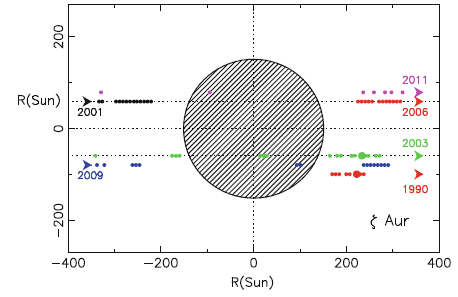
\includegraphics[width=0.6\linewidth]{Images/Geometria_eclipse.PNG}
    \caption{Geometría a escala de $\zeta$ Aur, que indica el seguimiento de seis eclipses. Las trayectorias modeladas se han desplazado verticalmente para mayor claridad, pero todas deberían estar a lo largo de la misma. Datos de 1990: espectros fotográficos del Calar Alto Observatory; y otros: espectros CCD del DAO.}
    \label{fig:geometria}
\end{figure}

\noindent En el caso del binario $\zeta$ Aur no solo se pueden conocer parámetros fundamentales, sino que son aún más relevantes porque como también se conoce la inclinación orbital, se puede obtener el valor de las masas dadas por la solución de órbita, las cuales son valores reales, en lugar de mínimos de una solución. De acuerdo a \citep{bennett1995non} la relación de masas es de $q = M_1/M_2 = 1.21 \pm 0.02$ con masas individuales de $M_K = 5.58 \pm 0.02 M_\odot$ y $M_B = 4.8  \pm 0.02 M_{\odot}$. Además, dado que los radios y las luminosidades de las estrellas componentes también pueden derivarse de una combinación de fotometría y espectroscopia, se pueden hacer coincidir sus posiciones en el diagrama H – R con las pistas evolutivas calculadas \citep{schroder1997critical} para sus masas correspondientes, lo que proporciona una verificación muy valiosa de los parámetros y supuestos que la teoría de la evolución ha adoptado.

\noindent En la actualidad, se tiene un principio de que los sistemas binarios tienen un potencial único como trazadores de la evolución estelar, permitiendo extrapolar características a estrellas individuales; Esto se basa en la condición de que la evolución de un miembro de un sistema binario no se ve afectada por su unión gravitacional a otra estrella, por muy distante que sea, como se indica en \citep{schroder1997critical}. Por lo que los modelos de cromosferas que se producen al analizar los eclipses atmosféricos de las estrellas Aur deberían ser representativos con respecto a otros gigantes. Sin embargo, aún hay preguntas que no han podido tener una respuesta satisfactoria; y con el estudio de líneas como la de Ca II y los cambios de ionización se pueden conocer si a pesar de enfoques diferentes relacionados con los vientos exteriores y cromósferas hay compatibilidades entre binarios e individuales.


\section{Espectroscopia Estelar}\label{espectroscopia}


\noindent Desde la antigüedad, nuestros antepasados se han preguntado por la composición de las estrellas que podemos observar en el firmamento. Gracias a la luz que nos llega de las mismas, actualmente podemos conocer la respuesta a esta y muchas más incógnitas planteadas muchos años atrás, ya que la espectroscopia es una de las herramientas más útiles en el análisis de objetos astronómicos.
\vspace{2mm}

\noindent Newton fue el primero en usar la palabra espectro al referirse a los colores en que se descompone la luz blanca al pasar por un prisma. Posteriormente, el astrónomo, óptico y físico alemán Joseph von Fraunhofer, usó un espectroscopio para descomponer la luz proveniente del sol y además de ver un continuo de colores, se observó la presencia de líneas oscuras, como se observa en la figura (\ref{espectro_frauhofer}), pero Fraunhofer no pudo explicar este comportamiento \citep{von1823denkschriften}. Fue hasta el siglo XIX, que Gustav Robert Kirchhoff y Robert Wilhelm Bunsen observaron que cuando los elementos químicos alcanzan ciertas temperaturas, emiten luz en longitudes de onda específicas, por lo que cada elemento tiene un espectro de líneas único y característico.

\begin{figure}[h]
    \centering
    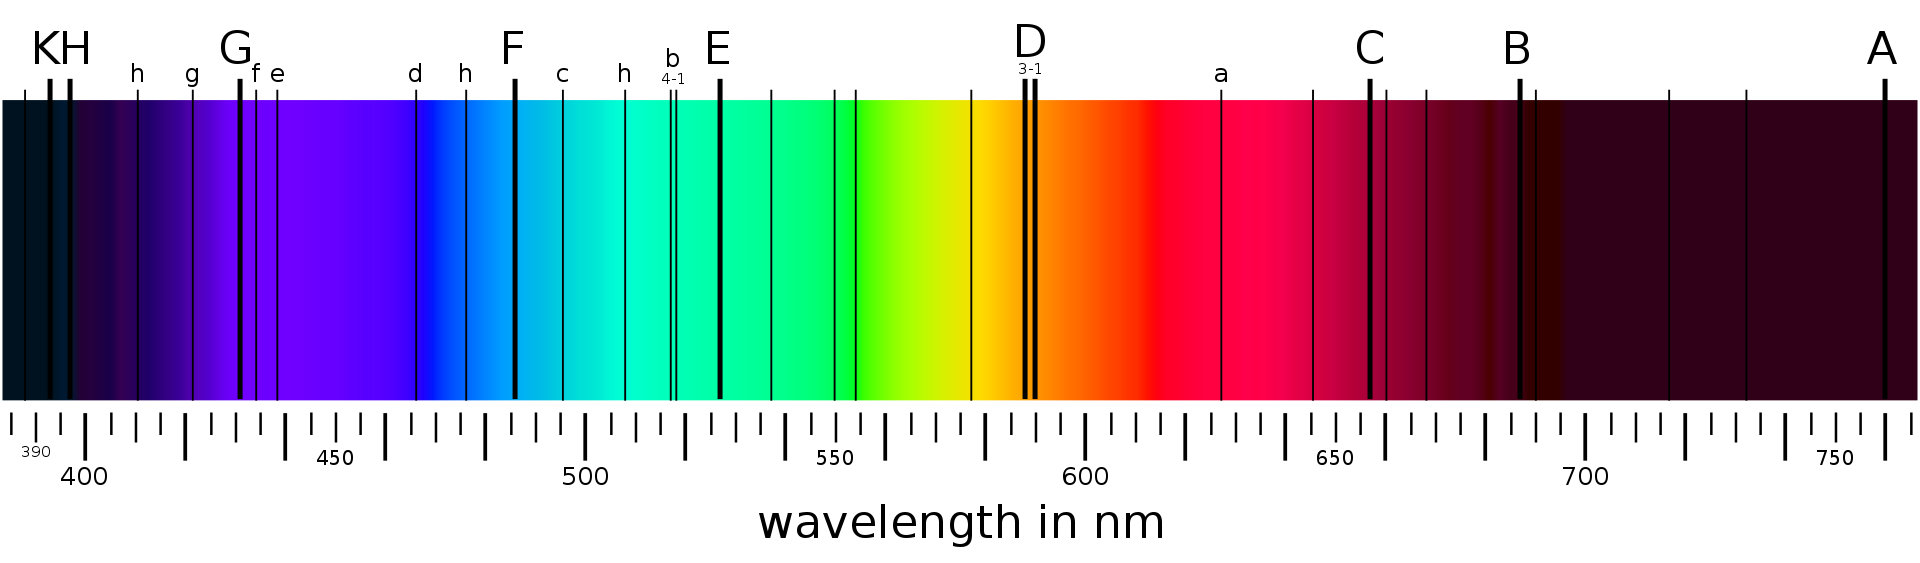
\includegraphics[width=1\linewidth]{Images/espectro_fraunhofer.png}
    \caption{Representación gráfica de las líneas de Fraunhofer. Dominio público, Wikimedia Commons.}
    \label{espectro_frauhofer}
\end{figure}

\noindent En 1886, el físico y astrónomo estadounidense Edward Pickering (1846 - 1919) en conjunto con su equipo (13 mujeres conocidas como calculadoras de Harvard) del Harvard College Observatory, retomaron un trabajo hecho por el astrónomo Angelo Secchi en 1874 que propuso una clasificación para las líneas espectrales. Contaron y clasificaron aproximadamente 225.300 estrellas, registradas en el \textit{Henry Draper Catalogue} \citep{gray2009stellar}; con lo cual hicieron el esquema de clasificación de Harvard de ``OBAFGKM'' con divisiones de 0-9, lo cual estaba relacionado con una temperatura, donde las estrellas tipo O, eran azules y calientes y las tipo M rojas y frías. Las primeras estrellas se conocen como tipo temprano y las cercanas al final como tipo tardío.
\vspace{2mm}

\noindent Posteriormente, al observar relaciones en los catálogos Henry Draper, en cuanto a temperaturas y además relaciones empíricas de masa-luminosidad dadas gracias a estudios en sistemas binarios, se encuentra que las estrellas O son mucho más masivas que las estrellas M. Lo que condujo a algunas teorías de evolución estelar. Posteriormente, los astrónomos Ejnar Hertzsprung y Henry Russell, llegaron a las mismas conclusiones, muy relevantes, pero trabajando independientemente, presentaron sus resultados, primero en tablas, pero al unir sus grandes contribuciones se llegó al célebre diagrama Hertzsprung-Russell o  \textit{diagrama H-R}. El cual registra las propiedades observables de una estrella, magnitud absoluta en el eje vertical (con el aumento de brillo hacía arriba) y el tipo espectral en el eje horizontal (con la temperatura aumentando hacía la izquierda) o índice de color. Este diagrama también permite hacer diferenciaciones de la masa de las estrellas de acuerdo a sus propiedades, por lo que se pueden hacer diferenciaciones como estrellas en secuencia principal (MS), Gigantes (G), Supergigantes (SG) y Enanas (D).
\vspace{2mm}

\noindent Teniendo en cuentas todas estas propiedades mencionadas anteriormente, se puede tener comprensión de la evolución estelar a partir de la secuencia de cambios dinámicos en el tiempo de las estrellas, desde la secuencia principal, de acuerdo a su masa inicial. Pero para entender mucho mejor los espectros enfocados a las estrellas es necesario conocer la estructura estelar, de dónde viene la luz que analizamos de las estrellas y cómo en su interior se forma esos espectros que posteriormente se van a analizar.


\section{Atmósfera estelar: Fotósfera}\label{sec:atm_est}
El modelo más simple para conocer la estructura estelar son capas esféricas superpuestas, dentro de las cuales se encuentra el núcleo estelar, la zona radiativa, zona convectiva, fotósfera, cromósfera, región de transición, y corona. La atmósfera que es en lo que nos vamos a detener a analizar, está compuesta desde la fotosfera hasta la corona, para algunas estrellas (como nuestro sol) y otras solo poseen fotosfera y cromosfera.
\vspace{2mm}

\noindent La fotósfera está compuesta principalmente de gas y una pequeña porción en forma de plasma o gas ionizado, el cual no permite que la luz pase, por lo que no es fácil conocer el interior de las estrellas, que es opaco; sin embargo el gas atómico o molecular da paso a la luz, lo cuál se conoce como continuo espectral y puede ser detectado por los telescopios, y es lo que forma lo que conocemos como espectro estelar, así que para interpretarlo, es necesario describir cómo viaja la luz a través del gas estelar. 



\noindent La cantidad de energía de una estrella viene dada por la ley de Planck, en la ecuación (\ref{ley_planck}), donde $h = \num{6.063e-34} [J]$, conocida como la constante de Planck, $k = \num{1.38e-23}$ $[JK^{-1}]$ es la constante de Boltzman, $c= \num{3e8} [m/s]$ es la velocidad de la luz en el vacío y $T$ la temperatura relacionada con la longitud de onda $\lambda$. Esta ecuación se relaciona con la \textit{radiación de cuerpo negro}, por lo que se pueden estudiar las estrellas como cuerpos negros, aunque esta presunción no es del todo cierta, los errores introducidos no son tan relevantes, sobre todo para estrellas de la secuencia principal.

\begin{equation}
    B(\lambda,T) = \frac{2h c^2}{\lambda^5} \frac{1}{e^{h c/k\lambda T}-1}
    \label{ley_planck}
\end{equation}

\noindent La ecuación (\ref{ley_planck}), se relaciona con la ley de desplazamiento de Wien, dada en la ecuación (\ref{wien}) para hallar su pico máximo. Donde $A = 0,0028976 [m\cdot K]$ se denomina la constante de Wien y $\lambda_{max}$ es la longitud de onda de máxima emisión.

\begin{equation}
    \lambda_{max} =  \frac{A}{T}
    \label{wien}
\end{equation}

\noindent Tomando nuevamente la presunción de que una estrella irradia isotrópicamente, entonces se obtiene la ecuación de Stefan-Boltzmann para un radiador ideal o un cuerpo negro, con el que se obtiene la energía radiada por unidad de tiempo y unidad de área, como se observa en la ecuación (\ref{stefan-boltzman}), donde $\sigma = \num{5,67 e-8}$ [W/m$^2$K$^4$] se conoce como constante de Stefan-Boltzmann.
\vspace{2mm}

\begin{equation}
    F = 4 \pi \int B(\lambda)  d\lambda = \sigma T^4
    \label{stefan-boltzman}
\end{equation}

\noindent En la figura  (\ref{fig:lineblanketing}) se observa cómo a pesar de analizar las estrellas como cuerpo negro es un buen modelo, este se usa más por su sencillez que por su exactitud, ya que las líneas de emisión y absorción de los espectros afectan el continuo en ciertas longitudes de onda, sobretodo en el canal azul, longitudes entre 3000 - 4000 [\r{A}], además también depende del tipo de estrellas que se esté analizando, para el caso de estrellas gigantes, que se caracterizan por su alta cantidad de metales, que por lo tanto hace que los espectros posean gran cantidad de líneas de absorción. Esta alta absorción, hace que se reduzca la intensidad del continuo y en ocasiones no se observen las líneas individuales. A este fenómeno se le conoce como \textit{blanketing effect} o \textit{line blanketing}, el cual hace una mejora de las regiones rojas o infrarrojas de un espectro estelar a expensas de las otras regiones, con un efecto general decreciente en las regiones azules del espectro.


\begin{figure}[h]
    \centering
    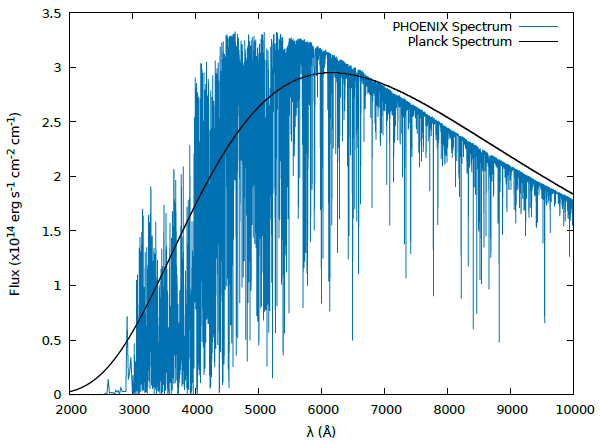
\includegraphics[width=0.9\linewidth]{Images/lineblanck.PNG}
    \caption{Comparación entre un modelo de espectro estelar a $T = 4700 K$ generado con el código PHOENIX, y una curva de cuerpo negro a la misma temperatura. La resolución del espectro se ha disminuido en un factor de 200. \textit{Tomado de \citep{Faiber2019master}}}
    \label{fig:lineblanketing}
\end{figure}

\noindent Desde la espectroscopia es muy importante tener en cuenta cómo medir las abundancias químicas en las atmósferas estelares (\textit{Este tema es explicado de manera más profunda en la sección \ref{sec:para_est}}), tanto para elementos neutros como ionizados; para lo cual teóricamente se implementan las ecuaciones de Boltzmann y de Saha para cada uno de los elementos, respectivamente.
\vspace{2mm}

\noindent Para describir la ecuación de Boltzmann, primero es necesario conocer la función de distribución de velocidades de Maxwell-Boltzmann, como se ve en la ecuación (\ref{eq:boltzmann}), la cual describe la fracción de partículas que están en un rango de velocidades $v + dv$, por unidad de volumen, además $n$ se refiere a la densidad total, $n_v = \partial n / \partial v$, $m$ es la masa de las partículas y $k$ la constante de Boltzmann.

\begin{equation}
n_{v} d v=n\left(\frac{m}{2 \pi k T}\right)^{3 / 2} e^{-m v^{2} / 2 k T} 4 \pi v^{2} d v
\label{eq:boltzmann}
\end{equation}

\noindent Ahora, los átomos de un gas, no solo tienen una velocidad caracterizada con la ecuación (\ref{eq:boltzmann}), sino  que también ganan y pierden energía a medida que chocan. Teniendo en cuenta estas dos características, es posible obtener una distribución de electrones definida entre los orbitales atómicos. Esta distribución de electrones se rige por un resultado fundamental de la mecánica estadística: es menos probable que los orbitales de mayor energía estén ocupados por electrones. Entonces se obtiene que la relación de probabilidades de que esté en un estado a y uno b está dado en la ecuación (\ref{ec:prob}), donde el término $e^{-E_{b} / k T}$ se conoce como factor de Boltzmann. 

\begin{equation}
\frac{P_b}{P_a}=\frac{e^{-E_{b} / k T}}{e^{-E_{a} / k T}}=e^{-\left(E_{b}-E_{a}\right) / k T}
\label{ec:prob}
\end{equation}

\noindent Hay que tener cuidado con los \textit{estados degenerados}, es decir aquellos estados en los cuales a pesar de que los números cuánticos del orbital a y b son diferentes, las energías son iguales; pues para estos casos cada estado degenerado hay que contarlo a parte. Por lo que ahora es necesario hablar de pesos estadísticos, $g_i$ los cuales están relacionados directamente con las energías y no con los números cuánticos, para así tener en cuenta todos los estados posibles.

\noindent En las atmósferas estelares hay una gran cantidad de átomos que tiene una rutina de probabilidades indistinguible; entonces, al aplicar estos métodos, tenemos que para los átomos de un elemento dado en un sitio de ionización específico, la tasa del número de átomos $N_b$ con energía $E_b$, con respecto a un número de átomos $N_a$ con energía $E_a$ en diferentes estados de excitación, conlleva a la ecuación de Bolztmann, aquí referenciada (\ref{eq:Boltzmann_real}).

\begin{equation}
\frac{N_{b}}{N_{a}}=\frac{g_{b} e^{-E_{b} / k T}}{g_{a} e^{-E_{a} / k T}}=\frac{g_{b}}{g_{a}} e^{-\left(E_{b}-E_{a}\right) / kT}
\label{eq:Boltzmann_real}
\end{equation}


\noindent Por otro lado, la ecuación de Saha asume equilibrio termodinámico, donde la tasa de electrones que caen es la misma con respecto a los expulsados, también sigue la distribución de velocidades de Maxwell-Boltzmann y se rige por poblaciones de niveles energéticos, teniendo en cuenta la ecuación de Boltzmann. Pero ahora, también se tienen en cuenta diferentes estados de ionización, donde $\chi_i$ es la energía de ionización requerida para arrancar un electrón del estado base. Llevándolo así de la etapa de ionización $i$ a $i+1$.

\noindent Esto lo vemos descrito en la ecuación (\ref{saha}) donde $Z(T)$ es la función de partición dependiente de la temperatura, $N_i^{ion}$ es un modelo de densidad de iones en función de la altura atmosférica y $T_{exc}$ es la temperatura de excitación.

\begin{equation}
A_{i} = \frac{\pi e^{2}}{m_{e} c^{2}} \frac{\lambda c}{v \sqrt{\pi}} g f \frac{N_{i}^{ion}}{Z(T)} e^{-E_{i} / k T_{exc}}
\label{saha}
\end{equation}

\noindent Teniendo en cuenta estás ecuaciones y los espectros obtenidos de una estrella, se puede conocer si las líneas de emisión o absorción son dadas en la fotósfera o en la cromósfera, de acuerdo a profundidad óptica, que en astronomía también se puede relacionar con un término conocido como la 'fuerza' de la línea.

\begin{comment}
un caso de estas líneas que no son producidas en la fotósfera como normalmente es esperado, son las líneas H y K, debido a la fenómenos físicos como la gravedad superficial $log(g)$ o la densidad de masa columnar $\sigma_{cm}$.
\end{comment}



\begin{comment}
\noindent Además, como las atmósferas no están compuestas de gas solamente de Hidrógeno sino que hay combinaciones e impactos que producen átomos más pesados como el Helio, pero en menor cantidad, normalmente 10 átomos H por cada 1 de He. Por lo que la presencia de otros átomos ionizados proporciona más electrones con los que los iones de Hidrógeno pueden volverse a combinar. Así que las temperaturas se van elevando para dar paso a este tipo de fenómenos.
\end{comment}

\subsection{Formación de líneas estelares}
En los espectros, se observa un continuo que es perturbado por líneas de absorción y emisión. Las líneas de absorción se crean cuando un átomo absorbe un fotón con exactamente la energía requerida para que un electrón realice una transición ascendente de un orbital inferior a uno superior; y las líneas de emisión se forman en el proceso inverso, cuando un electrón hace una transición descendente de un orbital superior a uno inferior y un solo fotón se lleva la energía perdida por el electrón.  Matemáticamente esto se puede escribir como en la ecuación (\ref{eq:energia_foton}). Además, la longitud de onda del fotón depende de las energías de los orbitales atómicos involucrados en estas transiciones, las cuales también se pueden distinguir aplicando las ecuaciones de Boltzmann (\ref{eq:Boltzmann_real}) y Saha (\ref{saha}). Por lo que cada línea espectral corresponde a una transición específica de un átomo en concreto. Las líneas nos permiten identificar los átomos presentes en la atmósfera de la estrella, y por tanto su composición química.

\begin{equation}
    E_{\gamma} = n(E_f - E_i) = h v = hc/\lambda
    \label{eq:energia_foton}
\end{equation}


\noindent Las distinciones entre los espectros de dos estrellas con diferentes temperaturas, se debe a electrones que ocupan diferentes orbitales atómicos en las atmósferas de cada estrella. Los detalles de la formación de la línea espectral pueden ser bastante complicados porque los electrones pueden encontrarse en los orbitales de cualquier átomo. Además, el átomo puede estar en cualquiera de las diversas etapas de ionización.

\noindent Ahora, para descubrir las bases físicas de la clasificación estelar se debe conocer la formación de las líneas de absorción y emisión pero para esto, también se debe conocer con claridad, la probabilidad de encontrar un electrón en un orbital para que este haga una transición y además conocer los números relativos de átomos de acuerdo a las etapas de ionización. Para esto, se cuenta con la rama de la física estadística, donde se analiza la \textit{opacidad}, la cual es una característica que tiene en cuenta cuatro fuentes primarias para eliminar fotones estelares de un haz: los cuales implican cambios de estado cuántico de electrones y los términos ligado y libre, que hacen referencia a si un electrón está unido al átomo o se trata de un ion en estado final o inicial.

\begin{itemize}
    \item[1.] \textbf{Interacción ligado-ligado} se producen cuando un electrón de un átomo realiza una transición de un orbital a otro y permanece ligado al átomo. De forma ascendente cuando gana energía por la apropiada absorción de un fotón, estás transiciones son responsables de líneas de absorción. En el proceso inverso, con transiciones descendentes, por volver al estado inicial o de menor energía, se emite un fotón y el resultado de esta secuencia es absorción-emisión. Si no vuelve a su estado inicial es una absorción pura. Si mientras está en un estado excitado tiene una colisión con una partícula vecina, lo que se convierte en parte de la energía térmica del gas, y genera degradación de la energía media de los fotones. No existe una única ecuación que tenga en cuenta todas estas posibles contribuciones.
    
    \item[2.] \textbf{Absorción ligado-libre}, también conocida como \textit{fotoionización}, ocurre cuando un fotón incidente tiene energía mayor a la energía de ionización, es decir, la suficiente para ionizar un átomo y arrancar un electrón. Cualquier fotón de $\lambda \leq hc/\chi_i$, donde $\chi_i$ es la energía de ionización del i-ésimo orbital; puede ser absorbido y esa energía se usa para arrancar un electrón del átomo. Esta absorción es continua, porque no se necesita una energía específica y puede producir una disminución de energía en el continuo espectral. 
    
    El proceso inverso sucede cuando el electrón libre se recombina con un ion emitiendo fotones en direcciones aleatorias y contribuye a reducir la energía promedio de fotones en el campo de radiación.
    
    \item[3.] \textbf{Absorción libre-libre} es un proceso de dispersión, cuando un electrón libre cerca de un ion, absorbe un fotón, lo que hace que aumente la velocidad del electrón; en este proceso, el ion cercano es necesario para conservar tanto la energía como el impulso. También puede pasar que al pasar cerca a un ion el electrón pierde energía al emitir un fotón, lo que hace que el electrón se desacelere, este proceso de emisión libre se conoce como \textit{bremsstrahlung}, que significa ``radiación de frenado''.
    
    Debido a estas dispersiones, los átomos en estado excitado que son inestables, por lo que luego el átomo se desexcita espontáneamente emitiendo de nuevo el fotón. Ese fotón a su vez lo vuelve a absorber otro átomo, y es vuelto a emitir, y así sucesivamente. Los fotones quedan de esta forma atrapados en la atmósfera y lo vemos evidenciado en las líneas de absorción.
    
    Como la fotosfera sigue aportando luz en todas las longitudes de onda, llegaría un momento en que los electrones capturados por una transición serían tantos que mantendrían todos los átomos excitados, como si estos fuesen estables. Los nuevos fotones emitidos por la fotosfera en esa longitud de onda ya no serían absorbidos, pues no tendríamos electrones en el nivel de energía bajo del inicio de la transición. Los fotones saldrían de la atmósfera, formarían parte del espectro, y la línea desaparecería. A este fenómeno se denomina \textit{saturación de la línea}.

    \item[4.] \textbf{Dispersión de electrones} es cuando un electrón dispersa un fotón a través del proceso de \textit{dispersión de Thomson}, es decir, el electrón oscila en el campo electromagnético del fotón. Sin embargo, como el electrón es pequeño, resulta en una pequeña región transversal, lo que significa que la dispersión electrónica es más efectiva cuando la densidad de electrones es muy alta, lo que requiere también una alta temperatura.
    \end{itemize}
    


%%%%%%%%%%%%%%%%%%%%%%%%%%%%%%%
%%%%%%%%%   Section   %%%%%%%%%
%%%%%%%%%%%%%%%%%%%%%%%%%%%%%%%




\subsection{Líneas fotosféricas características del sistema $\zeta$ Aur}





\noindent Una de las líneas más reconocidas de la estrella gigante del sistema $\zeta$ Aur es la línea H de Ca II. La formación de esta línea es muy particular ya que como se observa en la figura (\ref{fig:lineaCaii}) está compuesta por dos picos de emisión $K_2$ que se diferenciaran como pico azul, al derecho $K_{2B}$ y pico rojo $K_{2R}$, también se ven dos picos de absorción pura $K_1$ que al igual que en los picos rojos se llaman $K_{1B}$ y $K_{1R}$ y un último pico en medio que también es de absorción.


\begin{figure}[h]
    \centering
    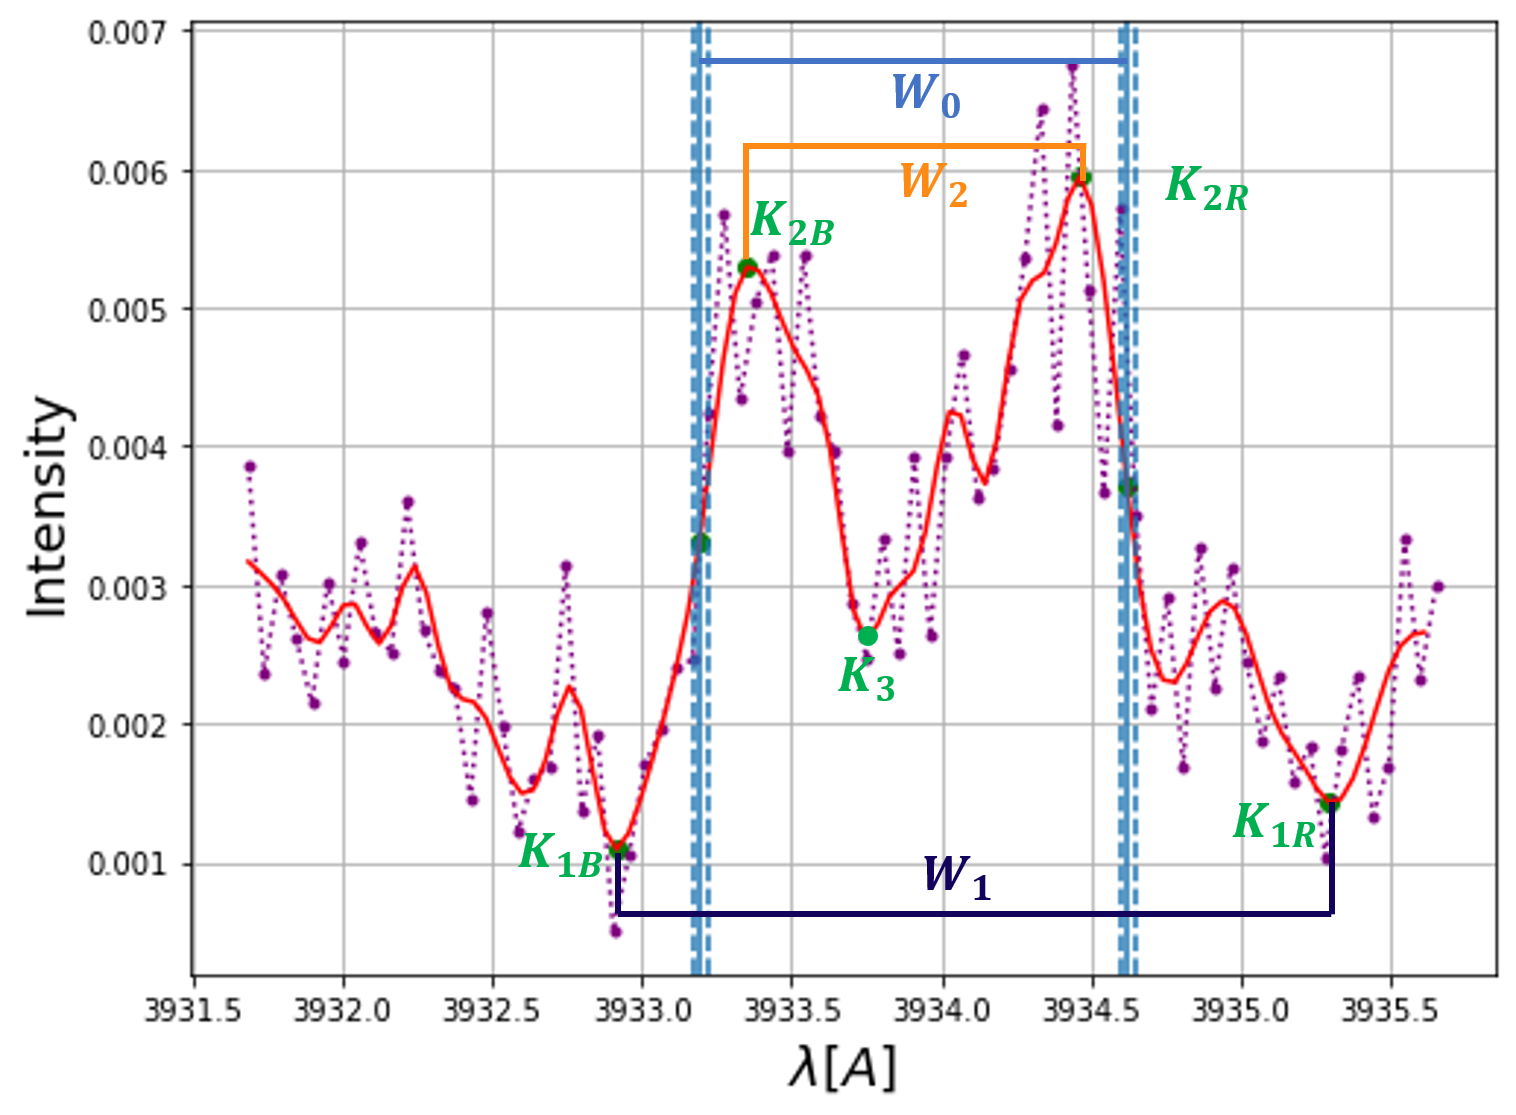
\includegraphics[width=0.8\linewidth]{Images/lineaCaii.png}
    \caption{Datos y ajuste por splines de la línea H de Ca II de la estrella gigante durante la totalidad del eclipse 2019}
    \label{fig:lineaCaii}
\end{figure}

\noindent La formación de los picos de absorción $K_1$ son generadas en la fotosfera y de acuerdo a que la temperatura en esta región de la atmósfera no es tan alta se puede asumir equilibrio térmico local y se genera porque el átomo gana energía por el impacto de un fotón haciendo que haya una transición a un nivel superior de energía y que al bajar de manera espontánea a su estado fundamental emite un fotón de la misma naturaleza que el absorbido. En esta zona de la fotosfera, según las ecuaciones de Saha y Boltzmann no se obtienen líneas de emisión. Por lo que ahora los picos de emisión $K_2$ son generados en la cromósfera baja según las ecuaciones de Saha y Boltzmann ya que se sigue cumpliendo el equilibrio termodinámico; solo que en este caso para que el átomo emita un fotón no es necesaria la absorción, sino que el átomo sube de nivel debido a energía térmica ya que las temperaturas en esta zona son más elevadas, pero se sigue cumpliendo la distribución de velocidades de Maxwell. Por último el pico $K_3$ se conoce como de autoabsorción, debido a que no es una absorción pura como en el caso de $K_1$, sino que este pico que se da en la cromósfera alta, donde ya no se cumple el equilibrio termodinámico, por ende tampoco se aplican las ecuaciones de Boltzmann y Saha se tienen átomos con electrones tan excitados y con una densidad electrónica tan baja que cuando hay impacto de fotones lo que se obtiene es un fenómeno de \textit{scattering} o dispersión.

\noindent Por otro lado, también se observa en la figura (\ref{fig:lineaCaii}) que esta línea no es necesariamente simétrica, pero estas formas aún hacen parte de estudios físicos ya que es bastante complicado de relacionar. Además el hecho de que el pico $K_3$ esté desplazado al azul, también se asocia a fuerte presencia de viento estelar o debido a simetrías no esféricas en el material cromosférico, según \citep{linsky1980stellar}.

Lo cual resulta un análisis muy importante y que nos puede brindar mucha información sobre la fotósfera de la estrella pero esto solo nos da información a una altura específica, que vendría estando dentro de la fotosfera, en cambio si se analizan otros elementos, desde otra perspectiva, es posible obtener información sobre resolución de diferentes altitudes, esto se puede lograr analizando específicamente el eclipse en diferentes fechas.


\section{Atmósfera estelar: Cromósfera}

Esta parte de la atmósfera solo puede ser observada durante los eclipses, y se le asemeja un color rojizo (que actualmente se conoce que se debe a la emisión de hidrógeno H $\alpha$ 656.280 nm). La cromosfera es aquella zona de transición que une la fotosfera y la corona (para las estrellas que la tienen).  Aunque en realidad la definición exacta de cromósfera en la actualidad no esta perfectamente detallada o delimitada en las alturas de la atmósfera. Inicialmente se podría mencionar como una capa atmosférica en la que hay una cantidad mensurable de calentamiento local además del transporte de calor radiactivo y convectivo que se tiene en la fotósfera; pero además también sería necesario incluir alguna distinción entre la cromosfera y la mucho más caliente corona que no emiten la línea H $\alpha$. 

Es posible establecer el límite inferior de la cromosfera por el signo del gradiente térmico de la atmósfera. Para esto, entonces la fotosfera sería la porción de una atmósfera estelar visible en luz óptica donde el continuo es ópticamente grueso, o casi, y donde la temperatura disminuye con la altura porque las fuentes de calor no radiantes no son lo suficientemente fuertes para modificar significativamente el equilibrio de la entrada de energía radiante y convectiva contra las pérdidas radiantes en el espacio. A cierta altura atmosférica, la combinación de el calentamiento no radiactivo y la disminución del enfriamiento radiactivo producto de la disminución de las fuerzas de densidad, hace que la temperatura aumente con la altura. Con esta definición física, se puede definir un límite inferior para la cromosfera a la temperatura mínima en la parte superior de la fotosfera y se extiende hacia arriba con el aumento de la temperatura. Debido a que las densidades son relativamente grandes en la parte superior fotosfera, el enfriamiento radiativo es muy eficiente, y la tasa de calentamiento no radiativo es mucho mayor que en las capas de menor densidad de la cromosfera. Como vemos entonces unas de las características más relevantes es el comportamiento de la temperatura y la densidad, las cuales van inversamente proporcionales, en la figura (\ref{perfil:densidad-temp}) se observan las variaciones en estas propiedades a través de la atmósfera. 


Ahora bien, también se ha observado que al variar la altura atmosférica o la profundidad óptica las líneas de absorción y emisión, son diferentes y cada unas se relaciona con diferentes mecanismos físicos que están sucediendo dentro de la atmósfera. Sin embargo, aún no es factible modelar ni siquiera la relativamente quieta atmósfera solar en toda su complejidad, los modelos de atmósferas actuales son buenas aproximaciones para ciertas regiones pero siguen siendo un importante estudio actual, hay mecanismos como en \citep{chavez2013new} y \citep{ayres2019stellar} donde  los campos magnéticos son cada vez más relevantes para explicar altas temperaturas a las que puede llegar la cromósfera y algunas de sus complejidades, pero aún hay puntos para que este sea un tema de discusión actual.

\begin{figure}[h]
    \centering
    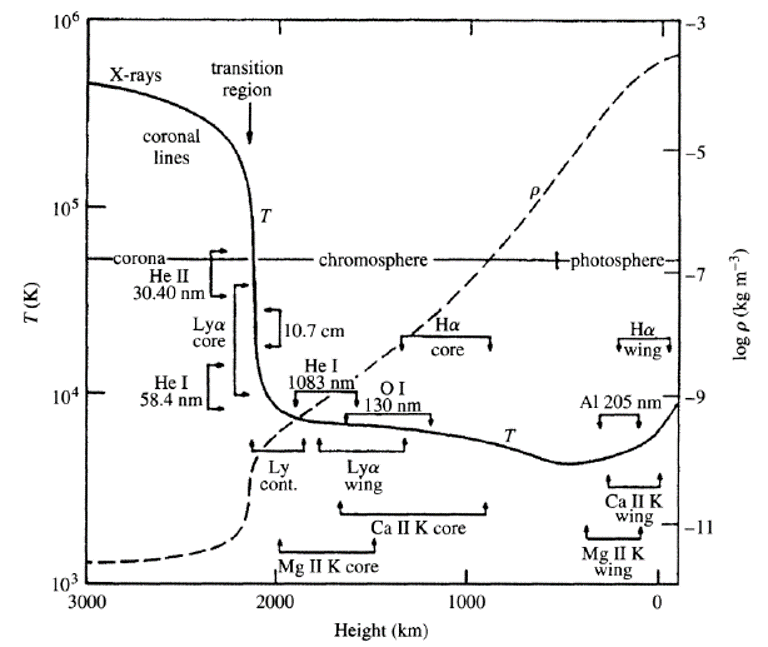
\includegraphics[width=0.8\linewidth]{Images/perfil_Densidad-temperatura.png}
    \caption{Perfiles de temperatura (línea solida) y densidad de masa (línea punteada) en relación con la altura de la atmósfera solar. Se muestra también las zonas de los perfiles donde se forman algunas líneas espectrales. Fuente \citep{carroll2017introduction}}
    \label{perfil:densidad-temp}
\end{figure}

Cabe también resaltar, que debido a las condiciones de la cromósfera, muchas de las aproximaciones no se pueden implementar debido a las condiciones que estas necesitan, como por ejemplo la ecuación de Boltzmann (\ref{eq:Boltzmann_real}) requiere de un equilibrio termodinámico para poder ser empleada y en la cromósfera esto ya no se da, debido a las altas temperaturas, por lo que en esta zona algunos de los resultados se pueden asociar a estructuras de campos magnéticos, según \citep{zhang2020magnetic}.

Normalmente no es tan sencillo diferenciar qué líneas son originadas en la fotósfera y cuales de ellas se originan en la cromósfera, pero de acuerdo a las temperaturas y los datos que se pueden obtener con el tratamiento de las líneas se podría saber las diferencias. Pero además para el caso de $\zeta$ Aurigae y otros sistemas eclipsantes se pueden obtener las líneas cromósfericas con una sustracción de espectros. Además a diferencia de las líneas fotosféricas que pueden tener un amortiguamiento notable, las líneas de la cromósfera se suelen caracterizar por ser más \textit{fuertes}.


\subsubsection{Espectros de la cromósfera del  sistema $\zeta$ Aur}

El espectro de la componente $\zeta$ Aur A (estrella gigante) se puede observar durante el eclipse total, es decir cuando la estrella $\zeta$ Aur B (estrella en secuencia principal) se encuentra oculta por completo. El espectro de $\zeta$ Aur B no se puede obtener de manera directa, pero si se puede recuperar mediante el proceso de sustracción punto a punto durante el eclipse parcial y el conocido eclipse de la componente $\zeta$ Aur A, con esto entonces obtenemos la suma del espectro B y las líneas de absorción cromosférica superpuestas, esto se puede observar en la figura (\ref{fig:espectro_zaur}).


\begin{figure}[h]
    \centering
    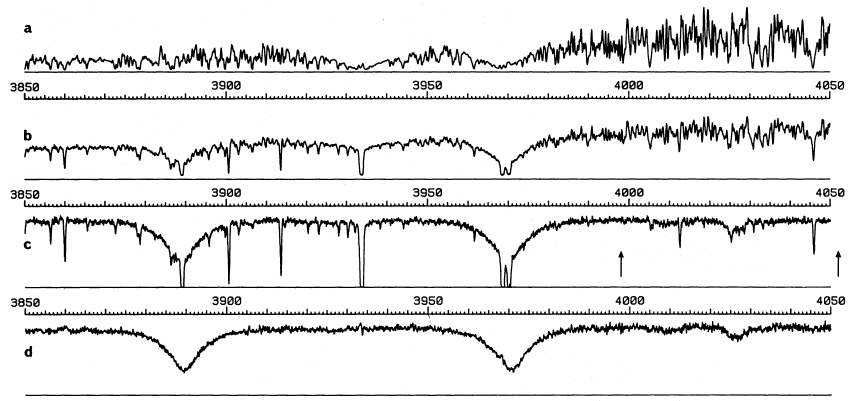
\includegraphics[width=1\linewidth]{Images/espectro_zeta_aur.PNG}
    \caption{Espectros en la banda B entre 3850 - 4050 \r{A} a) Espectro puro de la componente $\zeta Aur A$ durante el eclipse total b) Espectro compuesto del sistema binario durante el eclipse parcial c) Sustracción del espectro de la componente $\zeta$ Aur B y la superposición de las líneas de absorción cromosférica d) Espectro puro de la componente $\zeta$ Aur B \textit{Tomado de \citep{kps9}}}
    \label{fig:espectro_zaur}
\end{figure}

\noindent Además la figura (\ref{fig:espectro_zaur}) también se observan dos líneas características de las estrellas tipo tardío, referentes a calcio doblemente ionizado Ca II, la línea K de 3933.68 \r{A} y línea H junto a la línea H $\epsilon$ alrededor de 3968.47 \r{A}. 

Con esta figura se representa perfectamente el proceso de obtención de las líneas cromósfericas a partir de los espectros combinados para cada fecha durante el eclipse parcial, lo cual también se implementará en este proyecto de tesis y se explica con mayor detalle en la sección \ref{sec:sustraccion}.
%%%%%%%%%%%%%%%%%%%%%%%%%%%%%%%
%%%%%%%%%   Section   %%%%%%%%%
%%%%%%%%%%%%%%%%%%%%%%%%%%%%%%%




\section{Densidad de Masa columnar}
La densidad de masa columnar o densidad columnar es la cantidad de materia que recorre el fotón, pasando por la atmósfera en la línea de visión hasta el observador, matemáticamente se escribe como la integral de la densidad de masa volumétrica $\rho (z)$, la cual es radial y puede tener la forma de ley de potencias, %como en la ecuación (\ref{perfil-densidad})
también se describe como la cantidad de átomos de una misma especie en un área infinitesimal de atmósfera dependiente de la altura atmosférica a lo largo de la columna $dz$ como se observa en la ecuación (\ref{ec:denscolumnar}). Además en la figura (\ref{fig:rep_dens_masa}) se puede ver una representación gráfica de lo que se refiera esta magnitud, teniendo en cuenta las variaciones de temperatura y de densidad en la atmósfera.

\begin{equation}
    N = \int_a^b n (z) dz
    \label{ec:denscolumnar}
\end{equation}

\noindent Gracias a la espectroscopía, podemos conocer la densidad de masa columnar (N), ya que es una magnitud que afecta el ensanchamiento de las líneas espectrales, con esta se puede hacer un modelado estelar cromosférico, ya que si se obtiene N a partir de líneas de absorción pura que se forman en esta área de la atmósfera y se pueden obtener buenos modelos empíricos a alturas intermedias. Normalmente esto se hacen con líneas como Fe I, Ti II e H, según el tipo de estrella que se esté analizando, debido a que estas son líneas fuertes pero no saturadas. %Algunas de las características conocidas hasta la actualidad de esta magnitud es que hay una relación inversa con respecto a la altura y la temperatura.

\begin{figure}[h]
    \centering
    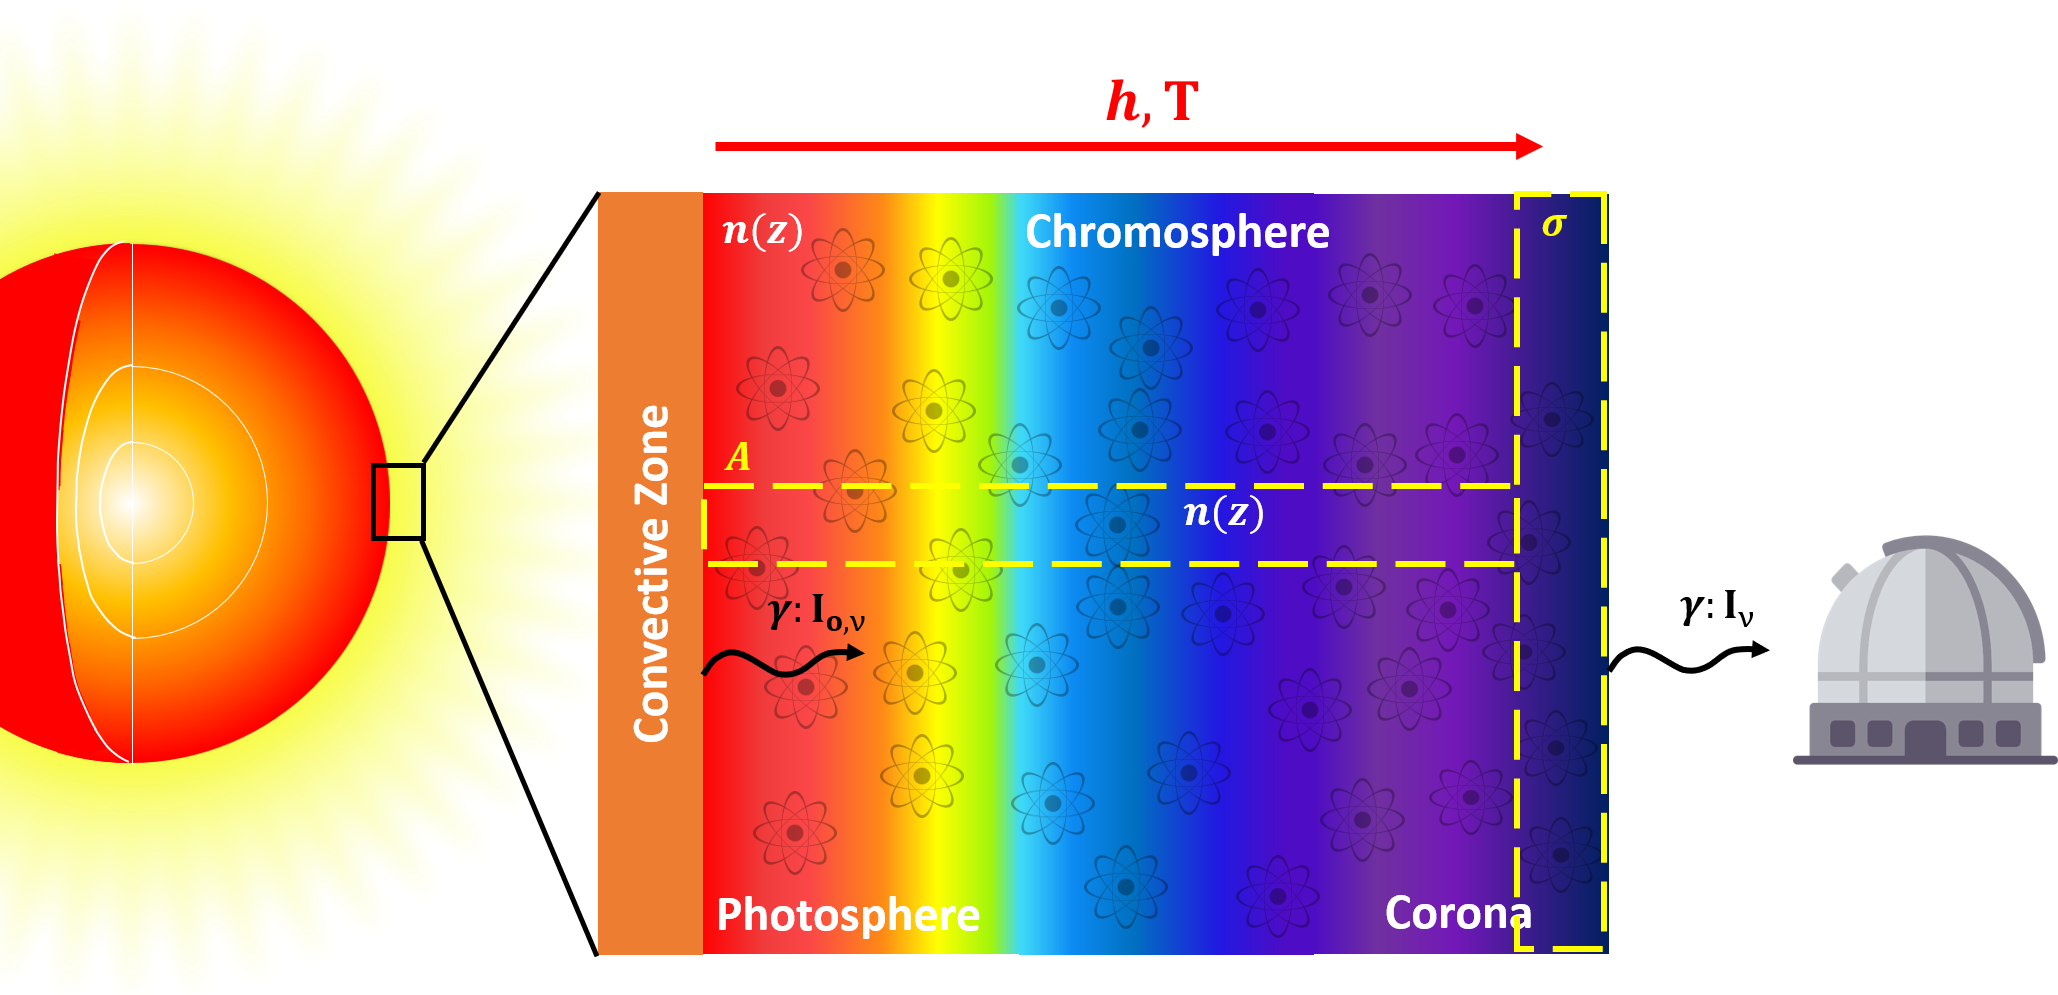
\includegraphics[width=1\linewidth]{Images/densidad_masa (2).png}
    \caption{Representación de la densidad de masa columnar en la atmósfera estelar}
    \label{fig:rep_dens_masa}
\end{figure}

Si aplicamos la ley de absorción pura simple, guiándonos con la figura (\ref{fig:rep_dens_masa}) un fotón que viene de la fotosfera con intensidad $I_{o, \nu}$, si sufre de absorción pura en el proceso paso por la atmósfera saldrá con una intensidad de la forma como en la ecuación (\ref{ec:ley_abs}) donde $\tau_{\nu}$ representa la profundidad óptica, que nos da una idea de la opacidad en cierta región específica.

\begin{equation}
    I_{\nu} = I_{o,\nu} e^{- \tau_{\nu}}
    \label{ec:ley_abs}
\end{equation}

La profundidad óptica se puede reescribir en términos de las características espectroscópicas que conocemos de las líneas como $\tau_{\nu} = \phi_{\nu} \tau_{o, \nu}$. Donde $\phi_{\nu}$ se conoce como la función del perfil de la línea que se relaciona con la forma de esta y sus \textit{wings}; además este nuevo $\tau_{o, \nu}$ se puede expresar en términos de la densidad de masa columnar y la sección de área transversal o las probabilidades de transición en átomos atómicos que absorbieron el fotón, como se expresa en la ecuación (\ref{ec:prof_opt}).

\begin{equation}
    \begin{array}{cc}
        \tau_{o, \nu} =& N \sigma \\
        \tau_{o, \nu} \propto& N fg
    \end{array}
    \label{ec:prof_opt}
\end{equation}

%%%%%%%%%%%%%%%%%%%%%%%%%%%%%%%
%%%%%%%%%   Section   %%%%%%%%%
%%%%%%%%%%%%%%%%%%%%%%%%%%%%%%%
\section{Curva de crecimiento}\label{CoG}

Como se había mencionado antes al analizar estrellas se quieren calcular las abundancias químicas que se encuentran en el interior de la atmósfera estelar. Uno de los métodos con que se pueden hacer esos cálculos es a partir de \textbf{anchos equivalentes ($W_{\lambda}$)}, que es una medida de la fuerza de las características espectrales, donde se tiene en cuenta la profundidad y el ancho de la línea respecto al continuo local. 

\begin{figure}[h]
    \centering
    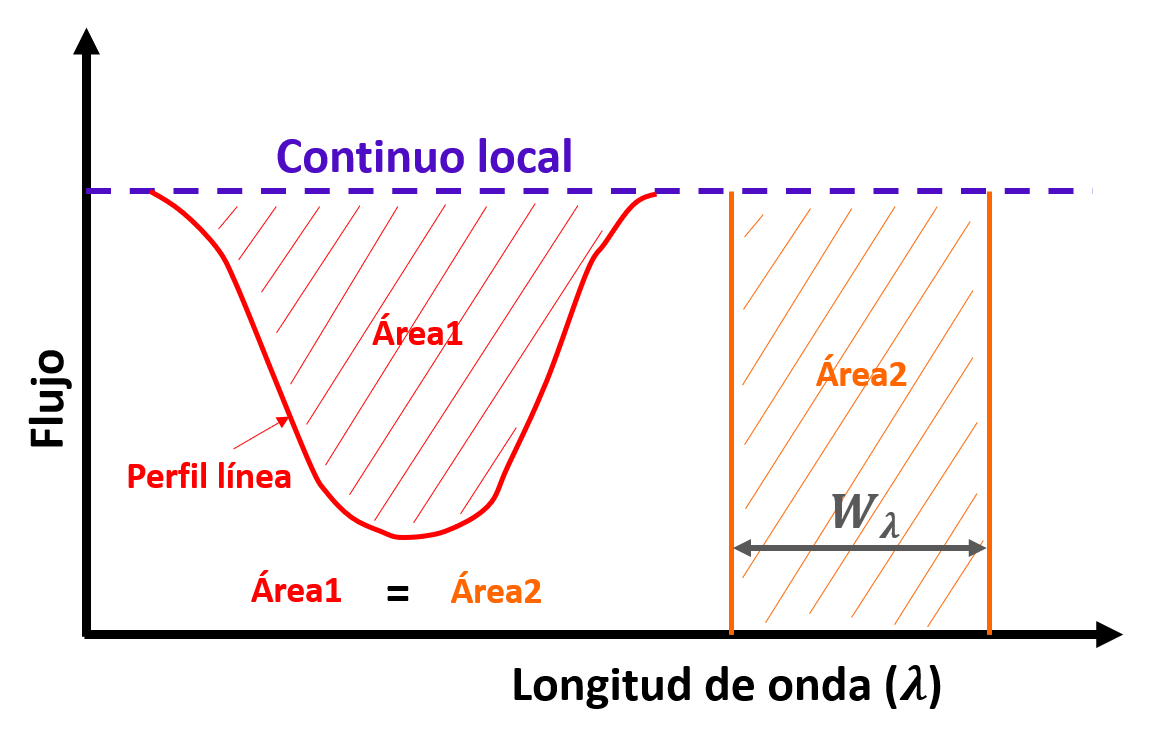
\includegraphics[width=0.6\linewidth]{Images/we.png}
    \caption{El ancho equivalente es el ancho de un rectángulo que tiene el mismo área que se encuentra dentro de una línea de absorción teniendo como referencia el continuo local}
    \label{fig:my_label}
\end{figure}

\noindent Para obtener información de la atmósfera estelar, se pueden crear curvas de crecimiento (CoG). Con estas curvas se quiere conocer cómo cambia el perfil de las líneas de un mismo elemento, es decir que tan pronunciadas son, en cuanto a su perfil de línea, lo cual se relaciona directamente con la profundidad óptica, la densidad de masa columnar y por ende el último concepto introducido, el ancho equivalente. Para esto, entonces un forma es graficar $log(W_{\lambda}/\lambda)$, en el eje \textit{y} y $log(gf)$ en el eje \textit{x}, donde $log(gf)$ son las fuerzas del oscilador, es decir, datos atómicos que dan información sobre la probabilidad que tienen los electrones de hacer una transición de un elemento específico de un orbital atómico a otro según la excitación y condiciones como la temperatura, entre otros. Cabe resaltar, que actualmente estos valores, para la astronomía se pueden extraer de repositorios de datos como ''Vienna Atomic Line Data Base'' (VALD) \citep{piskunov1995vald}, los cuales han sido obtenidos a partir de cálculos semi-empíricos, combinados con datos de laboratorio de alta precisión; esta base de datos tuvo su última actualización en el año 2019.

En la figura (\ref{fig:lines_cog}) podemos ver una representación gráfica de algunos tipos de línea que se pueden encontrar dentro de un espectro estelar, además cada una de estas de acuerda a estudios anteriores y como se registra en (\cite{carroll2017introduction}), donde se observan tres tipos característicos, las líneas fuertes, saturadas y \textit{damping wings}. Donde cada una de estas tiene una relación diferente entre el ancho equivalente (porque tienen perfiles diferentes) y la densidad de masa columnar o las probabilidades de transición, esto se observa en la ecuación (\ref{ec:relation_W_fg}) para cada una de estas líneas respectivamente.

\begin{figure}[h]
    \centering
    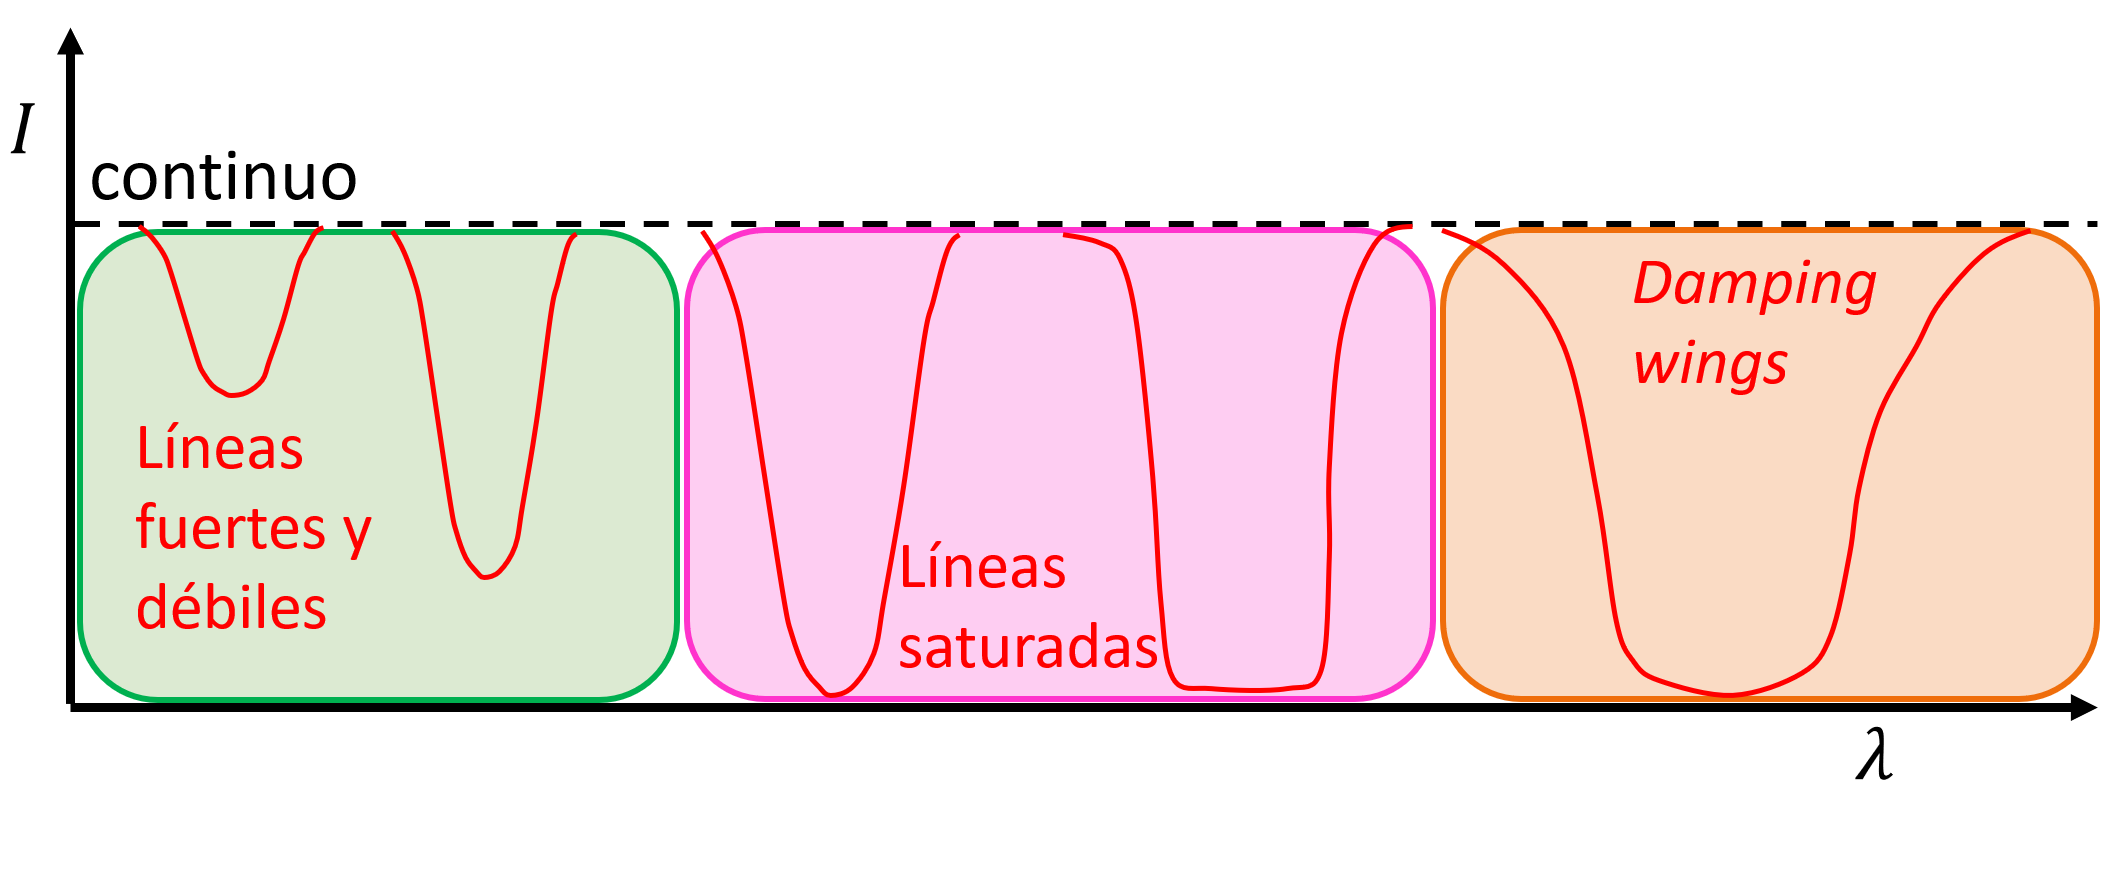
\includegraphics[width=0.9\linewidth]{Images/lineas_goc.png}
    \caption{Representación del tipo de líneas que se pueden encontrar en un espectro}
    \label{fig:lines_cog}
\end{figure}

\begin{equation}
    \begin{array}{cc}
         \frac{W_{\lambda}}{\lambda} \propto& Nfg\lambda  \\
         \frac{W_{\lambda}}{\lambda} \propto& log(Nfg)\lambda  \\
         \frac{W_{\lambda}}{\lambda} \propto& \sqrt{Nfg}\lambda
    \end{array}
    \label{ec:relation_W_fg}
\end{equation}

\begin{figure}[h]
    \centering
    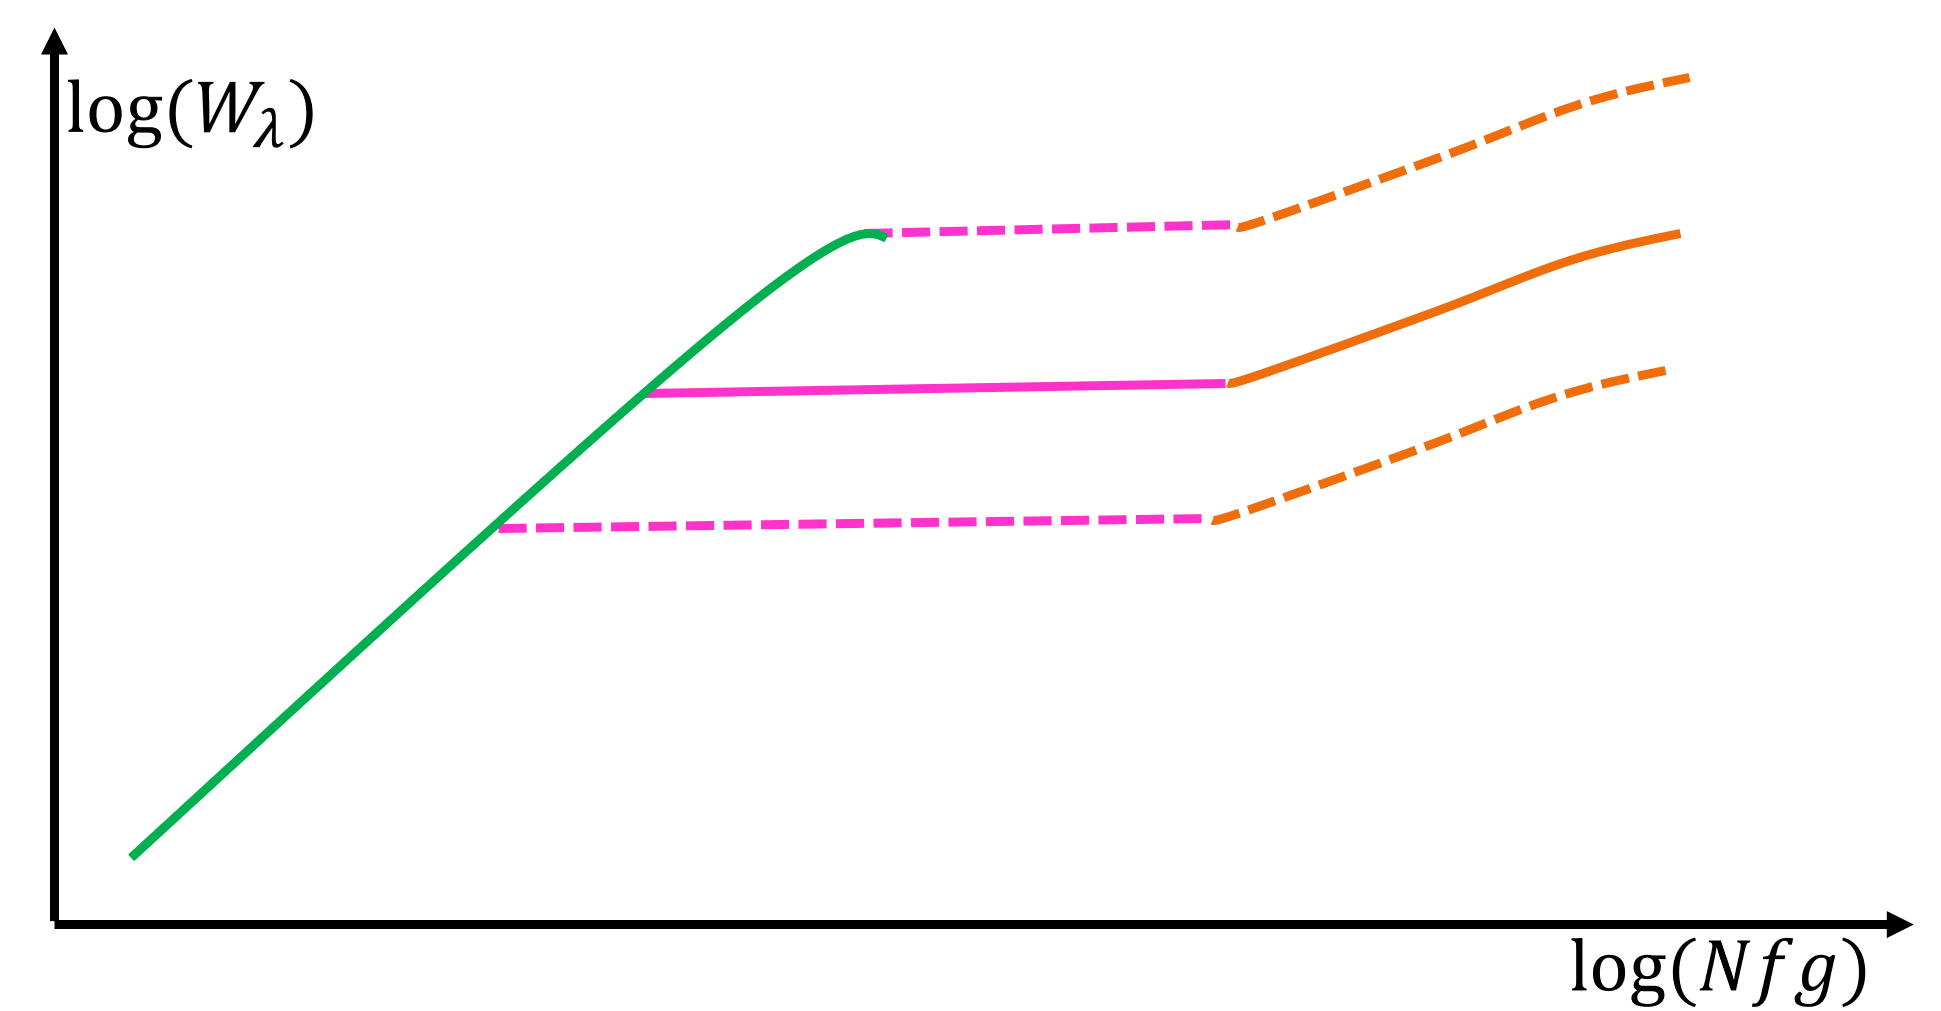
\includegraphics[width=0.75\linewidth]{Images/goc.png}
    \caption{Representación de Curva de crecimiento para un espectro con líneas fuertes, saturadas y con amortiguamiento en sus 'alas'.}
    \label{fig:GoC}
\end{figure}

Estas relaciones, evidencian que según las diferentes fuerzas de las líneas, como las de la figura (\ref{fig:lines_cog}) se tienen diferentes relaciones con la probabilidad de transición y el comportamiento de la densidad de masa columnar.  Una mejor manera de ver estas relaciones es con ayuda de las curvas de crecimiento. Por lo que en la figura (\ref{fig:GoC}) se representa una curva de crecimiento donde se tienen en cuenta los tres tipos de líneas en un mismo espectro. Vemos que para las líneas de absorción fuertes y débiles les corresponde una forma lineal, con pendiente 1:1, esto es debido a debido a la delgadez en la atmósfera. En el caso de líneas saturadas, vemos que varían los valores del eje x, manteniendo casi contante los valores de ancho equivalente, debido a la misma saturación; sin embargo se observa que esta puede darse para un rango de anchos equivalente mayor o menor y esto se relaciona directamente con la velocidad de turbulencia de la estrella. Para líneas fuertes o saturadas con presencia de 'alas' esta cuerva permite medir el amortiguamiento de la atmósfera; donde se observa que esta tiene una pendiente 2:1 y se le conoce como la parte del \textit{damping}.

\begin{comment}

\noindent Esta gráfica de \textit{CoG} experimental u observacional, también puede tener otros valores en el eje \textit{x}, como de densidad de masa columnar, ya que según lo vimos en la ecuación de Saha (\ref{saha}) estos valores son proporcionales.

Pero, esta curva, también se puede hacer teóricamente, ya que de acuerdo a perfiles de líneas gaussiano, lorentziano o deltas invertidos y según esto cada línea tendrá una intensidad que está dado por la ecuación (\ref{ec:intensidad_linea}) donde evidentemente depende de la longitud de onda $\lambda$, la longitud doppler $\Delta \lambda_D$ y la ecuación de Saha $A_i$, como se escribe en la ecuación (\ref{saha}) y se resuelve mediante integración numérica.

\begin{equation}
    I_i = I_0 exp\{-A_i e^{(\frac{\Delta \lambda}{\Delta \lambda_D})^2}\}
    \label{ec:intensidad_linea}
\end{equation}
\end{comment}





%Agregar se puede crear curva de crecimiento por elemento o curvas de crecimiento temporales, de todas las líneas en diferentes ocasiones.


%%%%%%%%%%%%%%%%%%%%%%%%%%%%%%%
%%%%%%%%%   Section   %%%%%%%%%
%%%%%%%%%%%%%%%%%%%%%%%%%%%%%%%




%%%%%%%%%%%%%%%%%%%%%%%%%%%%%%%%%%%
%%%%%%%%%%%%%% CHAPTER %%%%%%%%%%%%
%%%%%%%%%%%%%%%%%%%%%%%%%%%%%%%%%%%

\chapter{Datos Observacionales} : Instrumentación, adquisición y manipulación \label{cap3}
Debido a que en este proyecto se hace un análisis tanto teórico como observacional, se requiere del manejo de sets de datos, programas y scripts para la manipulación de los mismos. Por lo que es relevante conocer cómo han sido tomado los datos que se usan, qué repositorios de datos adicionales han sido requeridos y cómo estos se manipularon para hacer los respectivos análisis.

\noindent En este proyecto se usan datos de fotometría para definir con precisión las fechas exactas de ingreso y egreso del eclipse. También se usan datos de espectroscopia tomados por el telescopio TIGRE-HEROS para hacer el análisis de densidad. Además, también se usan datos de repositorios como del \textit{American Association of Variable Star Observers} (AAVSO) y la base de datos astronómica SIMBAD que proporciona datos básicos, identificaciones cruzadas, bibliografía y mediciones para objetos astronómicos fuera del sistema solar.

%%%%%%%%%%%%%%%%%%%%%%%%%%%%%%%
%%%%%%%%%   Section   %%%%%%%%%
%%%%%%%%%%%%%%%%%%%%%%%%%%%%%%%

\section{Fotometría}
Esta herramienta nos permite conocer el brillo de los objetos astronómicos, por lo que para sistemas binarios o planetarios es una herramienta fundamental, ya que según conocemos el mecanismo de un eclipse, observamos como hay un cambio en el brillo, durante el transito del eclipse. Con estas variaciones de brillo, podemos construir la gráfica conocida como \textit{curva de luz}, la cual muestra la intensidad de luz del sistema, en función del tiempo. Lo cual resulta útil, para conocer las fechas exactas de cada una de las fases del eclipse.
\vspace{2mm}

\noindent Para la gráfica de la figura (\ref{fig:curvaluz}), se usaron datos del repositorio AAVSO, específicamente se tomaron los datos de la banda azul, donde se usaron los filtros Jhonson B y Tri–color azul. En esta gráfica se puede observar que los valores constantes son debido a que la cantidad de brillo que llega a los detectores es constante mientras que en la parte lineal varía la magnitud, por ende hace referencia a etapas de contacto o fases parciales del eclipse.

\begin{figure}[h]
    \centering
    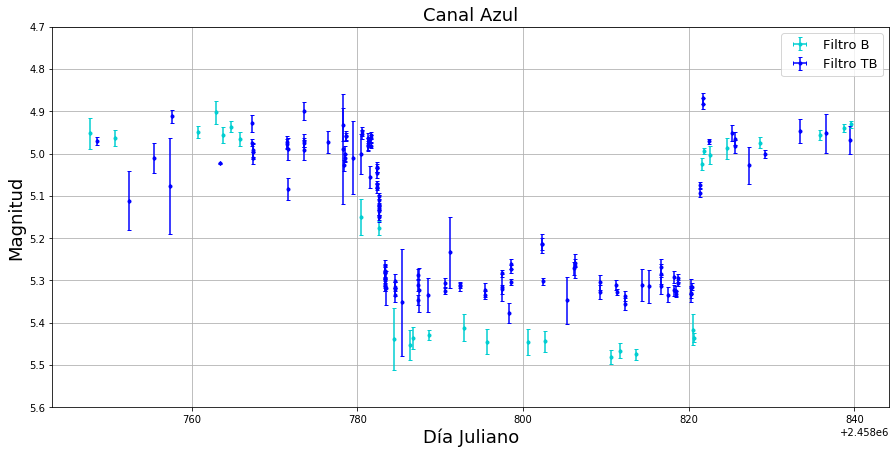
\includegraphics[width=1\linewidth]{Gaficas/curva luz.png}
    \caption{Magnitud aparente vs días julianos. En esta gráfica tenemos desde 21 Septiembre hasta el 22 Diciembre del 2019}
    \label{fig:curvaluz}
\end{figure}

\noindent Según esta figura (\ref{fig:curvaluz}), antes del 23 Octubre no hay contacto entre las estrellas, entre 24 - 26 Octubre es el primer contacto y la fase parcial entrante del eclipse; entre 27 Octubre y 2 Diciembre es el segundo y tercer contacto, es decir el eclipse total, momento en que solo se observa la estrella gigante ya que la de secuencia principal se encuentra por detrás según nuestra línea de visión. Además podemos observar que la entrada y la salida no duran lo mismo, porque la gráfica no es simétrica, por lo tanto nos muestra indicios de la excentricidad de la orbita; el cuarto contacto y fase parcial saliente dura tan solo dos días 3 - 4 Diciembre, así que a partir del 5 Diciembre de nuevo no hay contacto entre las estrellas.

\subsection{Altitud y proyección geométrica}

%%%%%%%%%%%%%%%%%%%%%%%%%%%%%%%
%%%%%%%%% Section  %%%%%%%%%
%%%%%%%%%%%%%%%%%%%%%%%%%%%%%%%
\section{Espectroscopía} 
La herramienta fundamental en este proyecto es la espectroscopia, por lo que dentro de la metodología resulta necesario explicar cómo se tomaron las datos, que incluye la instrumentación y cómo se van a manejar estos datos para obtener resultados favorables y cumplir los objetivos propuestos.

\subsection{Telescopio TIGRE - HEROS}

Como este proyecto está en convenio con la Universidad de Guanajuato en México y esta universidad cuenta con el telescopio TIGRE, por sus siglas Telescopio Internacional de Guanajuato Robótico Espectroscópico, el cual tiene un convenio bilateral con la Universidad de Hamburgo - Alemania y la Universidad de Liège - Bélgica, originalmente denominado ``Telescopio robótico de Hamburgo (HRT)'' en 2005, cuando fue entregado a la Universidad de Hamburgo para hacer pruebas.  Debido a limitaciones climáticas en el cielo alemán, el telescopio fue reinstalado en su sitio final, el Observatorio La Luz en septiembre de 2012, a una altitud de 2400 m sobre el nivel del mar en una meseta alta al norte de la ciudad de Guanajuato.

\noindent Este telescopio se concentra principalmente en física estelar. Tiene óptica Cassegrain-Nasmyth, el espejo primario tiene una apertura de 1.20 m, con distancia focal de 3.6 m, y el secundario alarga el foco a 9.6 m, por lo que es un sistema f/8, todos los dispositivos y software están diseñados para uso robótico remoto.

\noindent El observatorio TIGRE, también está conformado por un espectrógrafo, el cual para la calibración al telescopio se necesita un adaptador que alimente la luz de una estrella o de las lámparas de calibración. El telescopio se conecta con una fibra multimodo de sílice fundida con un diámetro de núcleo de 50 $\mu $ directamente al espectroscopio Echelle, con relación focal de f / 4.5 del colimador del espectrógrafo en su salida; como esta fibra tiene un largo de 15 m, ya que está ubicado en una habitación separada con clima controlado;  en su interior tiene microlentes integrales, basados en láser para minimizar las pérdidas de luz.

\noindent El espectrógrafo fue construido mediante la restauración del espectrógrafo HEROS (espectrógrafo óptico de rango extendido Heidelberg). Se tiene dos cámaras, una para el canal rojo y una para el azul, las cuales tienen un píxel de tamaño de 13.5 $\mu m$ por lo que precisión instrumental está únicamente por el ruido de lectura. Dentro del espectrógrafo, la luz primero pasa el colimador, luego por la rejilla echelle. Detrás de este último, se divide en dos haces de luz (luz azul y roja) a través de un divisor de haz dicroico.  El haz de luz azul cubre un rango de longitud de onda de $\approx$ 3750–5700 \r{A} y el haz rojo un rango de longitud de onda de $\approx$ 5830–8800 \r{A}.

\noindent El poder de \textit{resolución espectral} $\lambda / \Delta \lambda$ fue calculado con calibración de lámparas de ThAr de aproximadamente 20 000. Además, en cuando a \textit{relación señal a ruido} (SNR) depende de las condiciones climáticas y de la distribución de energía espectral de la fuente, pero según pruebas con estrellas estándar se mantiene superior a 100. 

\noindent Entonces los datos en su mayoría fueron tomados por este telescopio y espectrógrafo en las fechas comprendidas entre el septiembre y diciembre del año 2019 mientras ocurría el eclipse del sistema $\zeta$ Aur. Además estos datos fueron reducidos y estan en un formato en el cual por cada paquete de una fecha específica de datos hay cuatro archivos, el archivo $\_ main\_$ el cual contiene los datos, y el archivo $\_ small\_$ el cual contiene información relevante como las condiciones ambientales entre otros. Pero además como se había nombrado anteriormente hay datos del canal azul y del rojo. Estos archivos, los cuales son descargados directamente de la página de la Universidad de Hamburgo, están en formato \textbf{FITS}, que según sus siglas en inglés significa, Flexible Image Transport System, que en Astronomía es el formato estándar \citep{hanisch2001definition} de intercambio y archivo de datos.

\section{Reducción de datos}

Para hacer manipulación de los datos en el programa iSpec y en algunos códigos de Python, es necesario y facilita el trabajo usar archivos \textbf{.dat}. Por lo que es necesario hacer una conversión de los archivos \textbf{.fit}. Para esto se empleó un código llamado \textit{DataRedu}, el cual es una modificación de los archivos de conversión original creados en Hamburgo, los cuales se encuentran en el manual de usuario del Telescopio TIGRE-HEROS en la sección Software: \url{https://hsweb.hs.uni-hamburg.de/projects/TIGRE/EN/hrt_user/python_soft.html}. 
%Las modificaciones hechas en este código fueron hechas por mi codirector Faiber.

\noindent Estas modificaciones son muy eficientes ya que no es necesario pasar por cada uno de los paquetes de datos sino que está optimizado para que haga el trabajo con carpetas completas de datos, bajo algunas especificaciones. Además, genera un archivo que contiene el contenido del cuadro (\ref{Tabla:DataRedu}), el cual es muy útil para el uso de algunos códigos, ya que me muestra explícitamente cual es la resolución de cada uno de los sets de datos. Una explicación más detallada del funcionamiento y modificaciones está en el repositorio GitHub de este proyecto: \url{https://github.com/ntlucia/Tesis_Estrellas_binarias/tree/master/Scripts/DataRedu}.

\begin{table}[h]
\centering
\resizebox{15cm}{!} {
\begin{tabular}{|c|c|c|c|c|}
\hline
\textbf{SPECTRUM}                                     & \textbf{CHANNEL}                                                     & \textbf{RESOLUTION}                                                                               & \textbf{SNR}                                                               & \textbf{IRF}                                                                             \\ \hline
Nombre del archivo                           & \begin{tabular}[c]{@{}c@{}}Canal\\ rojo - azul\end{tabular} & \begin{tabular}[c]{@{}c@{}}Resolución del \\ telescopio y \\ espectroscopio\end{tabular} & \begin{tabular}[c]{@{}c@{}}Relación \\ señal a ruido\end{tabular} & \begin{tabular}[c]{@{}c@{}}Función de \\ respuesta \\ instrumental\end{tabular} \\ \hline
zetaAur-eclipse\_R\_2019\_11\_19\_02\_52\_08 & R                                                           & 20538                                                                                    & 496.82                                                            & 21.08                                                                           \\ \hline
zetaAur-eclipse\_B\_2019\_11\_19\_02\_52\_08 & B                                                           & 20652                                                                                    & 109.66                                                            & \textbf{}                                                                       \\ \hline
\end{tabular}}
\caption{Información de los espectros obtenida con el código DataRedu}
\label{Tabla:DataRedu}
\end{table}

\noindent Algo muy relevante de estos datos y el \textit{script} de reducción, es que se tiene la opción de hacer una corrección de flujo, para eliminar el continuo instrumental que no tiene relevancia física, en este se aplica la técnica denominada “rectificación del continuo” la cual es necesaria para poder hacer comparaciones y operaciones entre espectros. Pero como se observa en la figura \ref{fig:espectro_puro}, esta normalización no es muy confiable; en la región de 425 - 450 [nm] hay un pico que no corresponde con lo que se debería esperar (al compararlo con un espectro sintético de una estrella con los mismos parámetros estelares). Por lo que es necesario revisar con más detalle esta normalización, lo cual es mencionado en la sección \ref{sec:normalizacion} . Ya que al parecer las normalizaciones hechas por este código funcionan mejor para estrellas en secuencia principal y para el canal rojo, el cual tiene mayor SNR.

%en la figura pongo sin normalizar o continuo instrumental
\begin{figure}
    \centering
    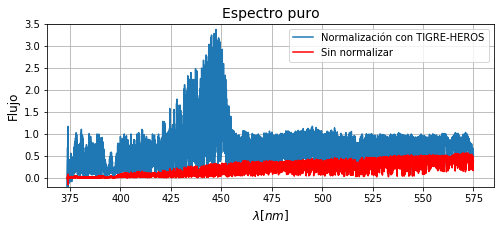
\includegraphics[width=0.9\linewidth]{Images/espectro_puro.png}
    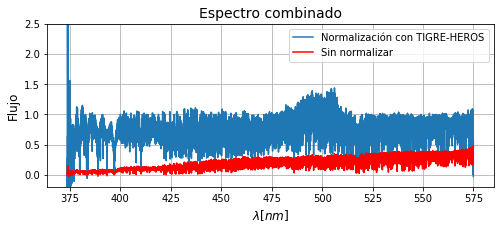
\includegraphics[width=0.9\linewidth]{Gaficas/espectro_combinado.png}
    \caption{Espectro puro de la estrella gigante roja del sistema binario Zeta Aurigae, el 19 de Noviembre del 2019 y espectro combinado durante el ingreso del eclipse, el 24 Octubre del 2019}
    \label{fig:espectro_puro}
\end{figure}

\subsection{iSpec: Parametros estelares}
\label{sec:para_est}

\noindent El programa iSpec es un programa basado en Linux, que también se puede instalar mediante Maquina Virtual, este programa, hecho por \citep{blanco2014determining} tiene la función de hacer análisis espectral y calcular parámetros físicos y estelares, teniendo en cuenta las especificaciones de la sección \ref{sec:para_est}. En el programa se tienen en cuenta códigos de transferencia radiativa, para crear espectros sintéticos o calcular abundancias por anchos equivalentes; Además este puede interactuar con otras aplicaciones como TOPCAT para graficar y y manipular catálogos astronómicos; VOSpec, para análisis espectral y fotométrico; y Splat para mostrar, comparar, modificar y analizar espectros. En general, con iSpec, se puede acceder al Observatorio Virtual (VO), que es un repositorio de datos de proyectos a nivel mundial.
\vspace{2mm}

\noindent El proceso de análisis se podría dividir particularmente en dos partes, para el canal azul y el canal rojo. Sin embargo, en este proyecto se hace un énfasis en el procedimiento del canal azul, ya que es donde se encuentran las líneas de absorción más pronunciadas. Inicialmente con canal rojo, debido a que tiene mejor SNR que el canal azul, como se observa en los ejemplos del cuadro (\ref{Tabla:DataRedu}), si se conocen los parámetros estelares teóricos, extraídos de Simbad \url{http://simbad.u-strasbg.fr/simbad/sim-basic?Ident=zeta+aur&submit=B\%C3\%BAsqueda+SIMBAD}, se puede hacer una verificación de que los espectros puros de la estrella gigante, por medio del cálculo de abundancias químicas estén en concordancia con lo encontrado en la literatura.

\noindent Para el cálculo de parámetros estelares y abundancias químicas es necesario hacer correcciones en longitud de onda $\lambda$ calculando la velocidad radial, ajustando un modelo de polinomios de segundo orden y ajustes gaussianos junto a una lista de mascaras de líneas llamada \textit{VALD.Sun.300\_1100nm} que se ajusta bien para este tipo de estrellas, como se observa en la figura (\ref{fig:vel_radial}) y posteriormente hacer la corrección con este valor de velocidad obtenido. Para la creación de un espectro sintético (sin líneas telúricas) y el cálculo de parámetros y abundancias; es necesario hacer el ajuste del continuo, por splines, en este caso, que no es una estrella solar y por lo tanto este tipo es más consistente según el ruido estocástico de los datos.

\noindent  Para sintetizar el espectro se tiene en cuenta el código \textit{TURBOESPECTRUM} el cual es un código de síntesis de espectro 1D LTE que cubre 600 moléculas, es rápido con muchas líneas y utiliza el tratamiento de ampliación de línea descrito por \citep{plez2012turbospectrum}; se usa el modelo de atmósferas \textit{MARCS.GES}, el cual tiene geometría esférica y el repositorio de abundancias \textit{GREVESS.2007} \citep{grevesse2007solar}. Adicionalmente, también se emplea la lista de líneas \textit{VALD.Sun.300\_1100nm}, que es una de las más actualizada y precisa para estrellas gigantes.



%\noindent Para el canal azul, se pueden identificar las líneas en el espectro para el gigante puro y ver cómo hay variaciones en algunas líneas. %MEJORAR MUCHO


\noindent Por otro lado, como lo que se quiere analizar son las líneas de absorción cromosféricas debido al eclipse, es necesario hacer una reducción de espectros y este programa lo permite hacer de manera práctica, donde se tiene el espectro puro de la estrella gigante durante el eclipse total, luego de ser analizado con las correcciones en longitud de onda e intensidad y también se tiene el espectro combinado en el ingreso y el egreso, por lo que estos se restan aritméticamente, con lo que se obtiene el espectro de las líneas cromosféricas superpuesto al espectro de la estrella estrella en secuencia principal.



\begin{figure}[h]
    \centering
    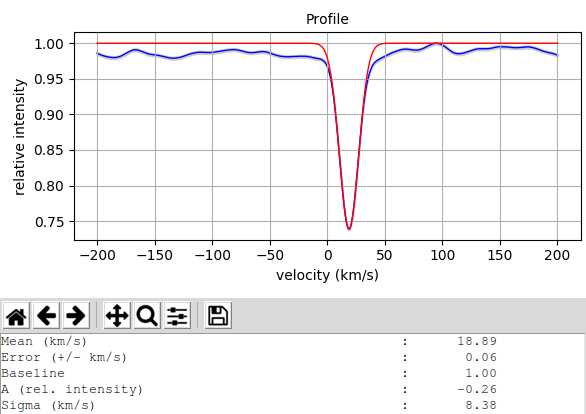
\includegraphics[width=0.8\linewidth]{Images/correct_vel_rad.PNG}
    \caption{Perfil de velocidad radial para hacer correcciones de longitud de onda}
    \label{fig:vel_radial}
\end{figure}



\noindent Teniendo en cuenta el espectro sintético, se puede normalizar el espectro observado por segmentos en los que no interfieran las líneas telúricas y adicional a esto proceder a calcular los parámetros estelares con este método de síntesis de espectro.

%%%%%%%%%%%%%%%%%%%%%%%%%%%%%%%%%%%%%%%%%%
\noindent A partir de la espectroscopia se pueden obtener abundancias químicas estelares, las cuales permiten conocer características de poblaciones estelares, patrones químicos y evolución química de elementos por canales de nucleosíntesis; esto depende principalmente de la muestra de estrellas que se analice, su masa y metalicidad. Para conocer estas abundancias hay que seguir una serie de pasos los cuales permiten conocer y analizar las atmósferas estelares y los parámetros que influyen en estas. 
\vspace{2mm}

\noindent Inicialmente lo primero que se debe tener claro es el tipo de estrella que se quiere analizar y de acuerdo a esto saber qué rango espectral se debe observar para obtener información relevante. Teniendo esto claro, es necesario que tener en cuenta las posibles incertidumbres que se puede tener y de acuerdo a esto conocer qué tan confiables son los resultados según los datos observados y la manipulación de los mismos.
\vspace{2mm}

\noindent Dos de las características más relevantes en los instrumentos con que se toman los datos son la \textit{resolución} y la relación señal a ruido (\textit{S/N}). Las cuales se deben buscar de acuerdo a lo que se quiere observar, por ejemplo, si se tiene baja resolución es positivo por el tiempo de observación requerido, pero si se quieren encontrar variaciones mínimas en estrellas u obtener perfiles de líneas de emisión o absorción se requiere de una alta resolución. Por otro lado, la S/N $>$ 200 da mucha confianza, pero comúnmente esta se encuentra entre 60-100 en telescopios terrestres y funciona para el tipo de estrellas FGK, S/N $<$ 40 ya comienza a ser incierto y S/N $<$ 20 ya no es confiable.
\vspace{2mm}

\noindent En cuanto a la manipulación de datos, es necesario hacer calibraciones en longitud de onda $\lambda$, teniendo en cuenta velocidades radiales. También es necesario eliminar líneas telúricas que pueden afectar el espectro debido a la luz proveniente de la estrella que al atravesar la atmósfera terrestre es absorbida y como esta está compuesta por moléculas, se observan líneas características que son dobles, repetitivas, fuertes y además en ciertas regiones del espectro. Según \citep{bertaux2014tapas} hay estándares o modelos telúricos con los cuales se pueden eliminar estas líneas que afectan el espectro, para evitar errores en la manipulación. Por último otro de los pasos y es uno de los que puede tener mayores incertidumbres, según \citep{jofre2017gaia} es la calibración en intensidades, la cuál se puede ver como la normalización del espectro, el cual se puede hacer por ajuste de splines o polinomios en regiones particulares sin tener en cuenta las líneas de absorción o emisión.
\vspace{2mm}

\noindent Ahora, no solo es necesaria la manipulación de datos, sino también entender a qué se debe la presencia de las líneas en el espectro, es decir, la formación de estas. Para conocer esta formación, es necesario tener en cuenta cálculos de transferencia radiativa debido a que las transiciones atómicas son muy complejos debido a la interacción de electrones con los campos de radiación, donde se tienen en cuenta excitación e ionización. Para esto, es necesario crear modelos de atmósfera en el que se suponga una estructura atmosférica y calcular las líneas espectrales estelares, por medio de perfiles gaussianos o perfiles de Voigt y con esto resolver ecuaciones de transferencia y hallar flujos continuos y netos. 

\noindent Para análisis de transferencia radiativa y modelos atmosféricos se puede por dos métodos principalmente, uno de ellos el \textit{Equilibrio termodinámico no local} (LTE), teniendo en cuenta la geometría y el equilibrio estadístico, sin embargo, las estrellas no son una ``caja ideal'' por lo que no se obtiene un solo flujo o temperatura, sino un rango de estos, así que hay que tener mucho cuidado con las delimitaciones que se hacen para conservar el equilibrio termodinámico. Otro método es por \textit{Tratamiento de opacidades por muestreo}, que es haciendo simulaciones hidrodinámicas de la atmósfera, donde se tiene un haz de luz paralelo y cualquier proceso que elimine fotones es absorción colectiva, donde se tiene en cuenta el scattering, la absorción real de fotones por transiciones de electrones atómicos y en gases frío por transiciones de nivel de energía molecular, es decir, lo que tenemos en cuenta es la \textbf{opacidad} la cual es función de la composición, la densidad y la temperatura. Según \citep{steffen2013micro} lo ideal es poder hacer análisis en 3D y no-LTE.

\noindent Teniendo en cuenta las geometrías, se pueden emplear principalmente dos, plana-paralela o esférica por capas, el cuál usar depende del tipo de estrellas que se está estudiando, para el caso de estrellas enanas es conveniente la primera, pero para estrellas gigantes, como se necesita tener en cuenta la curvatura de atmósferas extendidas es necesario usar la segunda. 

\noindent Una vez conocida la formación de las líneas, es necesario hacer un análisis de las líneas, para esto hay dos métodos principalmente y el uso del uno o el otro está relacionado al tipo de estrellas que se quieran analizar. Uno de ellos es por \textit{medición de anchos equivalentes en las líneas} (EW) y el otro es por \textit{síntesis de espectros}.

\noindent El primero es una medida del la fuerza de la línea, para esto se hacen ajustes a las líneas, por perfiles gaussianos para el caso de líneas débiles y perfiles de Voigt para líneas fuertes. Esta fuerza se relaciona con las abundancias, dados los parámetros estelares. Este método solo se puede usar para líneas débiles y fuertes ya que es la parte en la \textit{curva de crecimiento} que es lineal, en cambio para las líneas saturadas, se observa un plano, por lo que estas no brindan información relevante. Por otro lado, el segundo método, permite ajustar el espectro observado a un espectro sintético generado al variar parámetros y dejando el que menor $\chi^2$ tenga entre los dos y con este obtener valores con el menor error posible.

\noindent Por último, la relación entre la fuerza de la línea y la abundancia son los parámetros estelares, los cuales pueden ser \textbf{atmosféricos u otros} que también son necesarios, para explicar el ensanchamiento de las líneas y las escalas de abundancia. Según el catálogo PASTEL, \citep{soubiran2016pastel}, que es la compilación bibliográfica de parámetros atmosféricos estelares basados en espectroscopia de alta resolución y alta señal a ruido, se tienen límites, con los cuales ya no se puede obtener una mejor precisión. Estos parámetros son los siguientes:

\begin{itemize}
    \item[1.] \textbf{Temperatura efectiva ($T_{eff}$)}  se obtiene de la ley de Steffan-Boltzmann, con la ecuación (\ref{stefan-boltzman}), la cual se define de manera única para un nivel específico dentro de la estrella y es uno de los descriptores global importante de la estrella. Es muy importante no confundir esta deducción con la \textit{temperatura de excitación} la cual está definida por la ecuación de Boltzmann (\ref{eq:Boltzmann_real}), la \textit{temperatura de ionización} definida por la ecuación de Saha (\ref{saha}), la \textit{temperatura cinética} que se obtiene de la distribución de velocidades de Maxwell-Boltzmann (\ref{eq:boltzmann}) y la \textit{temperatura de color} que se obtiene del ajuste a la forma del espectro continuo de la función de Planck (\ref{ley_planck}). Estas otras temperaturas, diferentes a la efectiva tienen una posición específica en la atmósfera y varían según las condiciones del gas, que en el caso de gas ideal son la misma, debido a que las estrellas se asumen como cuerpo negro y con equilibrio térmico, por lo que una sola temperatura, las describe bien.
    
    \noindent Según las mediciones de este parámetro, la mejor precisión que se tiene de esta medida son 50 [K] y se puede calcular por diversos métodos como balances de excitación o interferometria.
    
    \item[2.] \textbf{Gravedad superficial (log[g])} es la aceleración gravitacional experimentada en la superficie del ecuador, incluidos los efectos de la rotación. Para esta propiedad, no se pueden hacer mejores mediciones que 0.1 dex, y se tiene una una dispersión promedio de 0.25 dex. Esta se puede medir por métodos como paralaje o ionización. 
    
    \item[3.] \textbf{Metalicidad} describe la abundancia relativa de elementos más pesados que el helio en la estrella, esta se puede escribir como [Fe/H] midiendo la abundancia de hierro con respecto a la del hidrógeno, pero no siempre basta con el hierro, sino que en ocasiones también es necesario tener en cuenta los metales en general, entonces es [M/H].

    \item[4.] \textbf{Microturbulencia ($v_{mic}$)} es otro parámetro relevante, la cual representa los movimientos turbulentos a pequeña escala que conducen con el ensanchamiento de las líneas, este no tiene exactamente un significado físico pero es necesario para dar explicación al ancho de las líneas.
    \item[5.] \textbf{Macroturbulencia ($v_{mac}$) y velocidad de rotación proyectada ($v sin[i]$)}, la  primera representa los movimientos turbulentos a gran escala en las atmósferas, como la actividad de la estrella, teniendo en cuenta excitación de átomos y movimientos de convección; la segunda hace referencia a la velocidad de rotación pero teniendo en cuenta la inclinación según el plano de observación. Estos dos parámetros realmente no son fácil separar, ya que sus contribuciones al ensanchamiento de las líneas es similar.
\end{itemize}


\section{Normalización de espectros}\label{sec:normalizacion}

\noindent La normalización del continuo puede ser una de las razones de mayor incertidumbre en el análisis de espectros estelares según \citep{jofre2017gaia}. Pero es muy importante, ya que el espectro rectificado es muy útil para comparar entre sí la profundidad relativa de las líneas espectrales, lo cual constituye un criterio fundamental en la técnica de la clasificación
espectral y además la obtención de abundancias y parámetros estelares. Así que es un tema bastante delicado, sobre todo porque para este proyecto es necesario hacer una sustracción de dos espectros, por lo que estos deben estar bien normalizados y así sustraer exactamente lo necesario de los espectros.
\vspace{2mm}

Cabe resaltar que la razón para que el espectro sea normalizado al continuo en cada orden, es para eliminar la forma que produce el espectrógrafo sobre la señal como se observa en la figura (\ref{fig:espectro_puro}). Esto puede ser observando las variaciones del flujo físico o haciendo una normalización en un valor constante según algún modelo específico como los mencionados en la sección (\ref{sec:para_est}), las líneas presentes en el espectro y el tipo de estrella u objeto astronómico que se analice.


\noindent Es necesario recordar que para este proyecto se tienen dos tipos de espectros característicos inicialmente, el espectro durante la fase de eclipse total que es el espectro puro de la estrella gigante roja y en las fechas de eclipse parcial tenemos el espectro combinado de la estrella gigante y la estrella en secuencia principal, por lo que en este último se tienen tanto líneas de la fotósfera como de la cromósfera de ambas estrellas. Por lo que estos se tienen que normalizar de manera diferente, ya que no es lo mismo manipular dato de una estrella en específico a la que le conocemos sus parámetros estelares gracias a la bibliografía; que trabajar con un espectro que tiene componentes de dos estrellas.


%No sé si sea necesario agregar si primero se hicieron pruebas probando la normalizació que tiene implicita el programa de ispec y ver cómo era y luego sí usando el programa cómo se pudo mejorar. Porque puede ser importante nombrar lo del pico de los 410 nm que es algo que según me comentaba Klaus también se vió ese problema que se reporta para el caso de 1989, que ahí solo se tuvieron en cuenta líneas hasta 4100 A, porque se veía un máximo 'artificial' que no debería ir y resultó ser un problema de normalización. que inicialmente también estabamos teniendo ese problema; pero ya con ispar lo logramos mejorar y ahora en esa zona se ve que sigue el mismo comportamiento.

Para realizar esta normalización, en este proyecto se implementa un script en Python llamado iSPar, que emplea funciones del programa iSpec, el cual tiene como fin último el cálculo de parámetros estelares, pero en este proceso implementa una normalización que se basa en la comparación con el espectro sintético. Por lo que funciona muy bien para el caso del espectro puro de la estrella gigante, tenemos espectros de una estrella en gigante roja, que por su etapa evolutiva tiene un espectro con grandes cantidades de metales presentes en ella y por lo tanto el efecto de \textit{line blanketing} descrito en la sección (\ref{sec:atm_est}) es muy evidente en regiones del espectro azul.

\begin{figure}
    \centering
    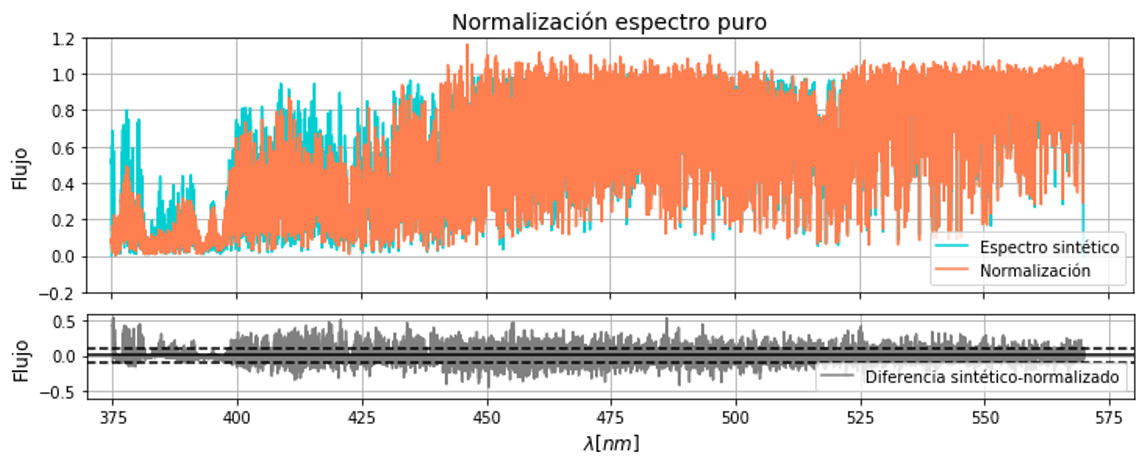
\includegraphics[width=1\linewidth]{Gaficas/comparacion_normalizacion.png}
    \caption{Comparación }
    \label{fig:normalizacion}
\end{figure}

Como vemos en la gráfica (\ref{fig:normalizacion}) para las regiones inferiores 450 nm no se puede tener un valor constante del continuo, sino que esa porción del espectro de la estrella parece reducida en flujo y se debe hay la gran cantidad de líneas de absorción por la presencia de metales. Ya que a pesar de que el espectrógrafo tiene una resolución de aproximadamente 20000 no se pueden estudiar todas las líneas individuales, sino que se reduce la intensidad del continuo.
%Además que al hacer comparaciones con el codigo PHOENIX, el espectro puro, tiene concordancia con esa caida en 400 nm para las estrellas gigantes como en este caso.

Para el caso del espectro combinado, obtenido durante el eclipse parcial, no se puede comparar con ningún espectro sintético, por lo que resulta mucho más eficiente hacer una normalización a un mismo valor, que en este caso por conveniencia, tomamos en uno. Esto lo logramos con el mismo script, variando como input el tipo de espectro que se ingresa y en el procedimiento lo que hace es %no me acuerdo.

%Agregar imágen



\section{Sustracción: Líneas cromosféricas}\label{sec:sustraccion}

Para obtener el espectro tan esperado de este proyecto, que es donde se tenga información de la cromósfera de la estrella gigante es necesario hacer una sustracción entre dos de los espectros mencionados anteriormente, uno de ellos es el espectro puro de la estrella gigante, que se obtiene del eclipse parcial, el cual a ser el espectro de una estrella "normal" como de cualquier otra, tiene información de toda la atmósfera estelar mezclada, es decir no es fácil solo con este espectro diferenciar qué efectos son provocados por la fotósfera y qué otros por la cromósfera. Así que aprovechamos el eclipse para obtener información más específica solo de la cromósfera.

Durante el eclipse parcial obtenemos información de la estrella gigante implícita mientras también se observa la absorción de la luz de la estrella en secuencia principal debido a la cromósfera de la estrella gigante, por lo que ahora si a esta información mucho más completa de la cromósfera se le resta el espectro de la gigante, donde se remueven todas las líneas fotosféricas se obtiene solo el espectro cromosférico combinado con las líneas de la estrella en secuencia principal, que no afectan en gran manera la información de la estrella gigante ya que sus líneas son muy anchas y características como las líneas de Balmer, por ser una estrella de esta región del diagrama H-R.

Pero además del proceso tedioso anterior de normalización, ahora hay que revisar exhaustivamente cuánto se debe sustraer espectro total, por lo que resulta necesario multiplicar por algún factor para que la profundidad de las líneas de ambos espectros sea coherente durante la sustracción. Si no se sustrae por completo, no es posible especificar que los resultados son solo para la cromósfera, si hay lineas de la cromosfera y de la fotosfera. Este factor multiplicativo, no es solo un factor escalar, sino que depende de la longitud de onda, porque de acuerdo al espectro de cuerpo negro que tenemos como base de cada una de las estrellas sus máximos no coinciden, por lo que hay longitudes de onda en las que la sustracción debe ser mayor o menor. Sin embargo, para regiones del espectro que no son tan amplios se puede asumir escalar.

Se hicieron pruebas de intentos/error para encontrar cuál era el factor que mejor se ajustado, inicialmente con la asesoría del experto en esta área de física estelar quién ha trabajado con espectros similares los últimos 50 años. Pero adicionalmente se implementó una rutina \textit{cross correlation} de python (scipy) para comparar el espectro puro de la estrella con solo el espectro sustraído con las líneas de la cromósfera.

Una vez verificada la correcta sustracción del espectro cromosférico, se observa en la figura () que ya no se obtiene un continuo en un solo valor, sino que ahora hay que trabajar con lo que se conoce como pseudo continuo o continuo local que viene siendo el flujo constante al rededor de cada línea individual que se va a analizar. Esto se debe a que desde la sustracción el espectro puro tenía sus disminuciones de flujo en la región $< 450 nm $, así que ahora el continuo se debe analizar localmente.



%CÓMO SABEMOS QUE YA LA SUSTRACCIÓN ESTÁ BIEN Y ESTÁ LIBRE DE LÍNEAS FOTOSFÉRICAS, Y CÓMO SE SABE SI UNA LÍNEA SE FORMÓ EN LA CROMÓSFERA O EN LA FOTÓSFERA???

Ahora, teniendo este espectro debemos identificar las líneas que se encuentran en él, que como ya mencionamos anteriormente solo se forman en la cromósfera. Para esto tomamos como base una lista de líneas publicada en () para este mismo sistema desde los 3650 hasta los 4600 A. De esta lista obtenemos la longitud de onda y el elemento con la que se relacionan, lo cual es muy importante para posteriormente obtener los datos atómicos correspondientes a estas lineas.

Una vez definidas no solo cuántas líneas hay en nuestro espectro (196) aproximadamente, debemos escoger de estas lineas realmente cuáles son pertinentes utilizar y para esto se tienen algunas restricciones: 
\begin{itemize}
    \item[1)] Deben estar dentro de los límites útiles, lo suficientemente fuertes para ofrecer una medición precisa, pero si pasar a ser líneas saturadas, es decir que su intensidad de absorción se extienda hasta cero o por debajo de este umbral,  como para perder información relevante respecto a la densidad. Algunos ejemplos de estos casos se observan en la figura (a, b). 
    \item[2)] Deben ser líneas sin mezclar. A medida que la línea de visión de la estrella B atraviesa capas cromosféricas sucesivamente más profundas, dan lugar a un espectro de líneas de absorción cada vez más rico; así que en algunos casos estas pueden estar mal resueltas debido a la resolución del espectrógrafo, un ejemplo de esto lo podemos ver en la figura (c), donde se observa la combinación de una línea de Fe I, junto con una de Ti II , por lo que no es certero identificar dónde comienza o termina cada una.
    \item[3)] Se debe encontrar una concordancia con la lista de valores atómicos que provee el repositorio VALD ().
\end{itemize}

Por otro lado, luego de aplicar estas restricciones nos quedamos con 100 líneas de absorción cromosférica; como con estas líneas se calculan sus anchos equivalentes y generan curvas curva de crecimiento, es necesario hacerlo con elementos que tenga varias líneas para poder hacer ajustes racionales, por lo que escogimos los elementos de Fe I, Ti II y Fe II, son los elementos con mayor cantidad de líneas funcionales en el espectro (36, 21 y 19 respectivamente).

\chapter{Curvas de Crecimiento}\label{cap4}
Como se explicó en la sección \ref{CoG} la importancia de las cuervas de crecimiento como un método para calcular la densidad de masa columnar, en este proyecto las usamos sobre el espectro de la cromósfera de la estrella gigante de este sistema binario, con las líneas explicadas anteriormente, es decir una curva de crecimiento por elemento mencionado. Para esto es necesario recordar que debemos hacer el procedimiento de calcular el ancho equivalente de cada una de las líneas y además obtener los datos atómicos que los relaciona, como la probabilidad de transición dada por el fuerza del oscilador y las energías de excitación entre los niveles transitorios.

%Falta agragar cómo se pusieron los límites a las líneas, de donde comienza y termina cada línea

\section{Anchos equivalentes y datos atómicos}
Para calcular los anchos equivalentes, inicialmente se usó la herramienta que tiene el código de ispec (fit lines determine ew and crossmatch with atomic data), haciendo pruebas con las diferencias variaciones posibles, como por ejemplo el tipo de perfil que se ajusta  a la línea: gauss o Voigt, lo cual mostraba comportamientos similares pero con valores diferentes, lo cual causaba inconformidades con lo que se debería obtener, teniendo como referencia algunos datos usado para la publicación (). Además revisando el código a profundidad se encontró que este código funciona tomando como referencia un continuo en 1, pero como lo vimos en la sección anterior este continuo es variable con la longitud de onda, así que esto podía estar introducciones errores que se evidenciaban en la alta dispersión de los datos.

Por lo que resultó necesario crear un código de cero que fuese recursivo y que hiciera todo el procedimiento de calcular los anchos equivalentes, teniendo como base la lista de líneas teóricas que se mencionó en la sección anterior (de 100 líneas)
pero que además de esto extraer los valores atómicos del repositorio de VALD correspondientes a cada una de las líneas, haciendo la restricción de las líneas del elemento específico que se se va analizar. La explicación de cómo se recomienda implementar este código esta explicado en el repositorio en github (\url{https://github.com/ntlucia/Tesis_Estrellas_binarias/tree/master/Scripts/Growth_curve})

Como inputs del código se tienen:
\begin{itemize}
    \item Archivo config.yaml, para editar la dirección de los archivos necesarios:
    \begin{itemize}
        \item Líneas teóricas de la cromósfera: contiene longitud de onda, elemento, límites donde comienza y termina la línea (\textit{wave\_peak, note, wave\_base, wave\_top} respectivamente)
        \item Lista de líneas atómicas provista por VALD: contiene longitud onda, elemento, loggf, energías de los dos niveles transitorios (\textit{wave\_nm, element, loggf, lower\_state\_eV, upper\_state\_eV} respectivamente)
        \item Espectro a analizar: contiene, longitud de onda, flujo y error de flujo (\textit{wave\_obs, flux, err respectivamente})
    \end{itemize}
    \item Elemento que se va a analizar escrito como el elemento y la ionización con un espacio entre ellos y como \textit{string}, por ejemplo: 'Ti 2', 'Fe 1'.
\end{itemize}

Como output, el código entrega un dataFrame listo para generar la curva de crecimiento, el cual contiene:
\begin{itemize}
    \item Pico de la línea, [nm] (wave\_peak)
    \item Extremo derecho, donde comienza la línea, [nm] (wave\_base)
    \item Extremo izquierdo, donde termina la línea [nm] (wave\_top)
    \item Elemento que se está analizando, si es el mismo quiere decir que hizo el \textit{match} con la lista de datos atómicos (note)
    \item Flujo asociado al pico de la línea (flux)
    \item Fuerza del oscilador, probabilidad de transición (loggf)
    \item Energía del nivel inferior en la transición (lower\_state\_eV)
    \item Energía del nivel superior en la transición (upper\_state\_eV)
    \item Ancho equivalente de cada línea (EWR)
    \item Error relacionado al ancho equivalente (errEWR)
    \item Error relacionado con el flujo del pico de la línea (error\_f)
\end{itemize}

Lo primero que emplea el script es relacionar las líneas que definimos como teóricas que se encuentran en el espectro cromósferico con el repositorio de datos atómicos de las transiciones espectroscópicas más usadas en el área de la astronomía (VALD), de acuerdo al elemento que se haya introducido que se analizará y extraer solo los de este elemento, ya que esta lista de datos atómicos contiene información de 731377 transiciones, así que para reducir tiempo de computo es mejor reducir esta lista. Pero no solo es necesario esta relación, sino también encontrar los valores reales y específicos que se tienen en en el espectro cromosférico, con todos sus decimales.

Teniendo conocimiento pleno de cuáles son los mínimos y los extremos límite de cada una de las líneas asociadas a un mismo elemento dentro del espectro, procedemos al cálculo de anchos equivalentes. Para lo cuál es necesario primero encontrar el continuo local para cada línea, ya que no es el mismo para todas. Para esto debido a que el error instrumental en $\lambda$ es de 0.03 nm (cita), asumimos que un ancho consistente es el doble en un factor adicional, es decir continuo de 0.6 nm a la derecha del extremo base y 0.6 nm a la izquiera del extremo superior, como se indica para un ejemplo, en la figura (). Entonces ese continuo local corresponde al promedio de los valores de flujo en ese rango mencionado anteriormente.


Ahora, como se observa en la figura () procedemos al cálculo de las áreas necesarias para obtener el ancho equivalente según la teoría descrita en la sección \ref{CoG}, para esto la primera área es la que está bajo el continuo dentro de los límites de la línea y a esta se le resta el área bajo la curva que se calcula como la integral de los puntos que conforman la línea, obteniendo el área dentro de la línea, que debe ser igual a la de un rectángulo desde el continuo local con el ancho equivalente que es el que estamos calculando. Por último como nuestra gráfica de curva de crecimiento es adimencional, dividimos entre las longitudes de onda del pico de cada línea y sacamos logaritmo base 10. (Todo el código se encuentra en el apéndice \ref{apendiceCoG} ).


\section{Observacionales y teóricas}

%%%%%%%%%%%%%%%%%%%%%%%%%%%%%%%%%
%%%%%%%%%%%% CHAPTER 5 %%%%%%%%%%
%%%%%%%%%%%%%%%%%%%%%%%%%%%%%%%%%
\chapter{Discusión: Comparaciones}\label{cap5}



%%%%%%%%%%%%%%%%%%%%%%
%%%%% CHAPTER 6  %%%%%
%%%%%%%%%%%%%%%%%%%%%%
\chapter{Conclusiones}\label{cap6}

%%%%%%%%%%%%%%%%%%%%%%
%%%%% CHAPTER 7  %%%%%
%%%%%%%%%%%%%%%%%%%%%%
\appendix
\chapter{Growth curve}\label{apendiceCoG}


\bibliographystyle{apacite}
\bibliography{propuesta}

\end{document}